\chapter{DESIGN AND VALIDATION OF SINGLE-ENDED Temperature and \ce{H2O} SENSOR }

\vspace{3mm}

\textit{Parts of this chapter is currently under review as Yuzhe Zhou, Garrett C. Mattews and Christopher S. Goldenstein, ``A compact, fiber-coupled, single-ended laser-absorption-spectroscopy sensor for high-temperature environments,'' Applied Optics (2018).}

\section{Introduction}
TDLAS sensors have been extensively used to acquire non-intrusive, in situ measurements of gas temperature, pressure and composition in many practical combustion environments and energy systems \cite{Goldenstein2017, Ma2013, Caswell2013,Stritzke2015,Bürkle2018, Witzel2013,Makowiecki2017,rieker2009calibration,Li2011}. Typically, traditional laser-absorption sensors, known as LOS-LAS sensors, rely on transmitting laser light across an unobstructed line-of-sight, however this approach is not suitable for some environments with extremely limited optical access or in situations where standoff detection is needed. To overcome this challenge single-ended laser-absorption-spectroscopy (SE-LAS) sensors have been developed, which rely on backscattering laser light off native surfaces \cite{Dubinsky1998,Wainner2002,Wang2015,Goldenstein:16,Peng:16,Peng2018} or surfaces within optical probes \cite{RIEKER20073041,Rein:10,Chen2010,0957-0233-25-11-115501,GIRARD2017158}. Recently, SE-LAS sensors have emerged as a promising approach to characterizing combustion environments with limited optical access \cite{Goldenstein2017}. While promising, all prior single-ended LAS sensing in combustors relied on the use of windows to isolate the SE-LAS sensor from the high-temperature combustion gases. This increases sensor cost and complicates sensor installation since care must be taken during alignment to avoid collecting strong reflections off the window surface which can significantly compromise the accuracy of single-ended LAS sensors.

The design and validation of a compact single-ended laser-absorption-spectroscopy (SE-LAS) sensor for measuring temperature and $H_2O$ in high-temperature combustion gases ($\approx 1000\,K$) is presented in this thesis. The design presented here builds on the fiber-coupled SE-LAS sensor developed previously by Goldenstein et al. \cite{Goldenstein:16} to provide several design improvements which increase the practicality and applicability of laser-absorption sensors without compromising measurement quality. 1) The sensor presented in this thesis is a windowless (in addition to a lens) single-ended LAS sensor which can withstand direct exposure to high-temperature combustion gases. 2) The SE-LAS sensor presented in this thesis use a 18$x$ smaller lens to provide a 9$x$ smaller footprint (compared to \cite{Goldenstein:16}) which enables this sensor to be integrated into environments with tighter spatial constraints. 3) A simple approach for reducing the computational time required to perform scanned-WMS spectral-fitting by a factor of 100 is presented. This enables large datasets to be processed in a reasonable amount of time using personal computers and could facilitate the integration of scanned-WMS-2f/1f techniques into stand-alone sensors.

In this chapter, the architecture of this sensor is demonstrated including experimental setup and sensor housing design first. Then the diagnostics techniques are described with an accelerated scanned-WMS-$2f/1f$ spectral-fitting routine first applied. This section is followed by the demonstration and evaluation of SE-LAS sensor's performance in a propane-air burner including: i) collection efficiency of SE-LAS sensor, ii) comparison of the SE-LAS sensor measurement with that of a traditional LOS sensor and iii) uncertainty analysis of the measurements.

\section{Diagnostic Techniques}
The sensor presented here is demonstrated using first-harmonic-normalized wavelength-modulation spectroscopy with second-harmonic detection (WMS-$2f/1f$) techniques. WMS-$2f/1f$ techniques where the nominal wavelength is fixed (fixed-WMS-$2f/1f$) or scanned (scanned-WMS-$2f/1f$) in time were both used. The former was used to provide measurements with greater bandwidth to resolve an ignition event, while the latter was used to provide greater measurement accuracy via spectral-fitting techniques that avoid the need for knowledge of collisional-broadening coefficients \cite{Goldenstein2014}. These methods and their relative attributes have been described in the previous chapters.

\subsection{Line selection}
Water has been a popular monitoring species in TDLAS for combustion diagnostics \cite{Goldenstein2017}. Accuracy of TDLAS relies on the appropriate line selection, the rules of which have been developed for measuring uniform gas in low-pressure applications \cite{Zhou2005}. Generally the criterion for the line selection includes the linestrength, temperature sensitivity and isolation from neighboring transitions. Strong transitions can give a large gain in detector signals and thus great precision with low SNR. The temperature sensitivity depends on the difference of lower-state energy between two selected transitions, which is give by Eq. (4.1). This work employs near-infrared wavelengths near 1343 nm and 1392 nm to investigate the combination and overtone absorption bands of $H_2O$ utilizing robust semiconductor lasers and telecommunication-grade fiber optics \cite{FURLONG1998103}. These wavelengths were used to interrogate two strong and well-characterized $H_2O$ doublet transitions due to their large strength, isolation from interfering transitions, and disparate lower-state energies (see Table.4.1), the latter of which enables sensitive thermometry at the temperatures of interest here. These wavelengths have been used extensively to characterize combustion environments via TDLAS and some prior works \cite{Goldenstein:16,Goldenstein2014,rieker2009calibration,strand2015quantification} are recommended for greater detail regarding the suitability and performance of LAS sensors employing these wavelengths in combustion systems.

%($\nu_1+\nu_3$ band) ($2\nu_1$, $\nu_1+\nu_3$ band)

\begin{equation}
|\frac{dR/R}{dT/T}|=(\frac{hc}{k})\frac{|E_1^"-E_2^"|}{T}
\end{equation}

\begin{table}[h]
\begin{center}
\begin{tabular}{ c c c c }
\hline
Species & $\nu_0$ $[cm^{-1}]$ & $S(296 K)$ $[cm^{-2}/atm^{-1}]$ & $E^"$ [$cm^{-1}$]\\ \hline
$H_2O$ & 7185.59 & 0.0196 & 1045\\ 
$H_2O$ & 7446.35/.37 & 0.0011 & 1774/1806\\ \hline
\end{tabular}
\caption{Wavelength, linestrength and lower-state energy of the two color transitions used in this work \cite{Goldenstein:16}}
\label{table:ch4_1}
\end{center}
\end{table}


\subsection{WMS-$2f/1f$ model and simulation techniques}
A model capable of predicting WMS-2f/1f signals as a function of gas temperature, pressure, and composition is required to convert measured WMS signals to measurements of gas conditions. These models consist of sub-models for: 1) the absorbance spectrum of the target species and 2) each laser’s wavelength and intensity modulation.
Absorbance spectra of the selected transitions were calculated using the algorithms presented in \cite{GOLDENSTEIN2017249}. Simulations were performed using the HITRAN2012 database \cite{2013JQSRT.130....4R} in combination with the experimentally validated linestrength and collisional-broadening parameters. Fig. 4.1 shows simulated absorbance spectra for the relevant wavelength region at conditions representative of the propane-air burner operating at quasi-steady state (1000 $K$, 1 $atm$, $10\%$ $H_2O$ by mole). 

For simplicity, fixed-WMS-2f/1f signals were simulated using the calibration-free WMS model developed by Rieker et al. \cite{rieker2009calibration}. This model requires knowledge of the wavelength-modulation depth ($a_m$), $1^{st}$ and $2^{nd}$-order intensity modulation amplitudes ($i_0$, $i_2$), and the phase shift between wavelength and intensity modulation ($\psi_1$, $\psi_2$). The laser-modulation parameters were determined according to the methods described in \cite{rieker2009calibration}.

Typically, this simulation technique has been directly integrated in a least-squares fitting routine with the integrated absorbance ($A$), collisional width ($\Delta\nu_C$), and transition linecenter frequency ($\nu_0$) as free parameters \cite{Goldenstein:16,Goldenstein2014,goldenstein2014scanned,spearrin2014simultaneous}. The parameters corresponding to the best-fit spectrum are then used to calculate gas properties. While accurate, this approach is computationally expensive, typically requiring 10$s$ of seconds (using MATLAB's function $nlinfit$ on a modern personal computer) to find the best-fit scanned-WMS-$2f/1f$ spectrum for a single measurement. The following subsection presents a simple solution to reducing computational time by using a pre-calculated library of scanned WMS-$2f/1f$ spectra.

\begin{figure}  
\begin{minipage}[h]{0.5\linewidth}  
\centering  
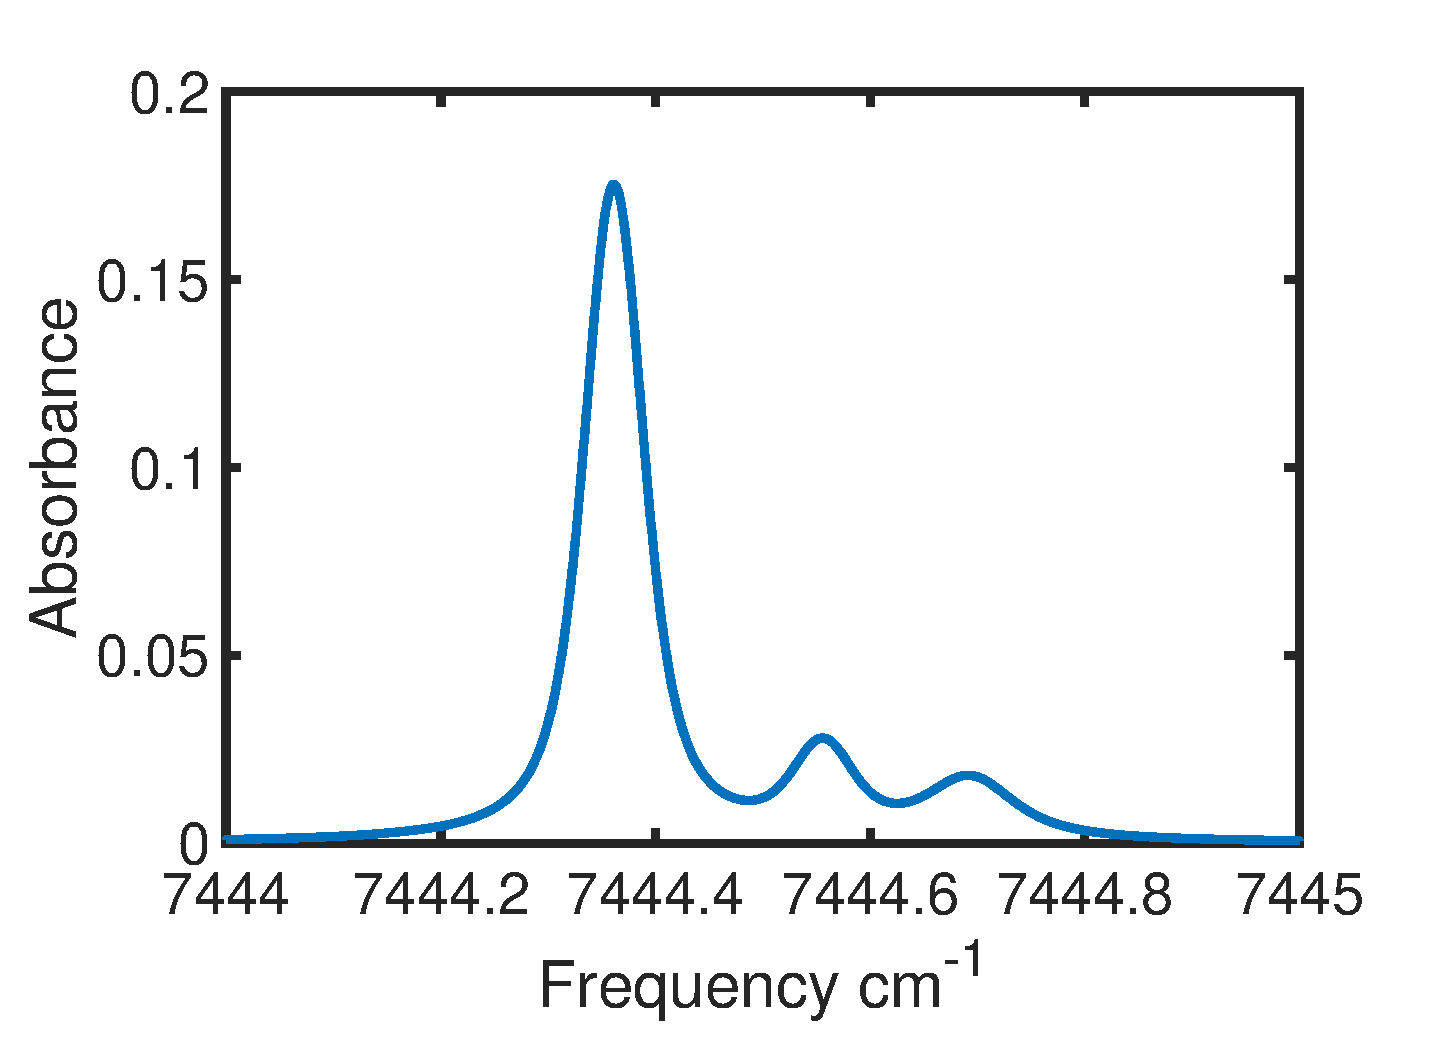
\includegraphics[width=1\textwidth]{fig/ch4_fig3_1.eps}  
\end{minipage}%  
\begin{minipage}[h]{0.5\linewidth}  
\centering  
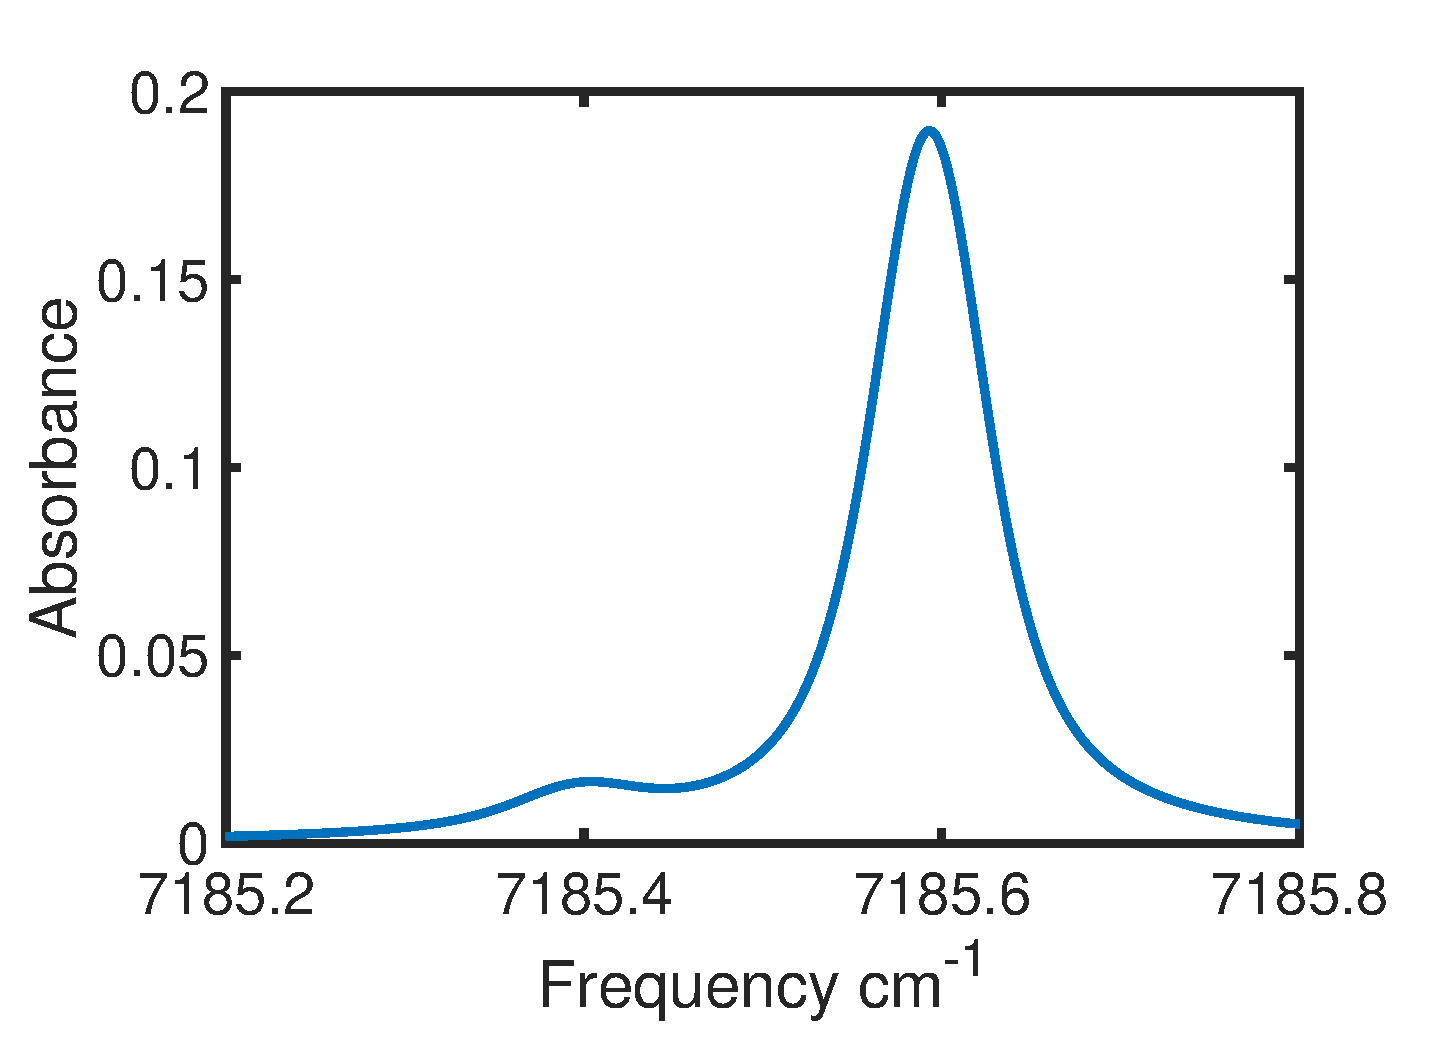
\includegraphics[width=1\textwidth]{fig/ch4_fig3_2.eps}  
\end{minipage} 
\caption{Simulated absorbance spectra of the H2O transitions targeted by the SE-LAS sensor. Simulations performed for a gas at 1000 K and 1 atm with $10\%$ $H_2O$ by mole and a path length of a 7.52 cm.}
    \label{fig:ch4_3}
\end{figure} 


\subsection{Accelerated scanned-WMS-{$2f/1f$} spectral-fitting technique}

To reduce the time required for data processing, a library of scanned-WMS-$2f/1f$ spectra was generated for a given spectroscopic model and set of laser-modulation parameters. It is worth noting that the use of look-up tables to accelerate spectral-fitting routines is a common approach in broadband techniques (e.g., hyperspectral absorption and coherent anti-Stokers Raman scattering), however this has not been used previously in scanned-WMS-$2f/1f$. As a result, the primary value of this work is: 1) describing what level of resolution (within the look-up table) in each spectroscopic parameter is recommended for a given measurement accuracy and 2) quantifying the reduction in computational time associated with this approach. The scanned-WMS-$2f/1f$ simulation technique developed by Goldenstein et al. \cite{Goldenstein2014} was used to simulate scanned-WMS-2f/1f spectra corresponding to each laser and each absorption transition of interest for a fixed Doppler width, $\Delta\nu_D$ (set by the temperature of interest), and numerous values of $A$, $\Delta\nu_C$, and $\nu_0$. Each simulated scanned-WMS-$2f/1f$ spectrum corresponding to a unique combination of $A$, $\Delta\nu_C$, and $\nu_0$ is then stored in a 4-dimensional array, illustrated as a “data block” in Fig. 4.2, with each cell containing a scanned-WMS-$2f/1f$ spectrum spanning a pre-determined frequency/wavelength range (set by the laser scan amplitude, $a_S$). Spectra corresponding to the up-scan and down-scan of the laser’s wavelength are stored separately, since they differ for the same thermodynamic conditions due to the phase shift between the laser’s intensity and wavelength response \cite{Goldenstein2014}.
The resolution of each dimension of the data block (i.e., of each spectroscopic parameter) should be chosen to provide the level of accuracy and precision desired by the user and the size of the library should be large enough to span the range of expected gas conditions. Further, for cases where the Lorentzian-to-Doppler width ratio is near unity, a unique library for every 200 $K$ change in temperature is recommended to account for changes in the Doppler width, although the user should confirm that this provides the desired level of accuracy. For the experiments presented here, the dimensions and resolution of the library were chosen to yield an accuracy of $\approx 1.5\%$. The specific dimensions of each library used here are shown in Table.4.2.

\begin{table}[h]
\begin{center}
\begin{tabular}{ c c c }
\hline
Parameter & Laser: 1392 $nm$  & Laser: 1343 $nm$ \\
 & Min:step:Max & Min:step:Max\\ \hline
$\nu_0$,$cm^{-1}$ & 7185.58:0.001:7185.60 & 7444.34:0.001:7444.36\\ 
$A$,$cm^{-1}$ & 0.022:0.0005:0.035 & 0.015:0.0005:0.0275\\ 
$\Delta\nu_c$,$cm^{-1}\cdot atm^{-1}$ & 0.06:0.00075:0.1 & 0.045:0.00075:0.075\\ \hline
\end{tabular}
\caption{Resolution of spectroscopic parameters used to generate scanned-WMS-$2f/1f$ spectra in the look-up table used by the accelerated scanned-WMS-$2f/1f$ spectral-fitting routine.}
\label{table:ch4_2}
\end{center}
\end{table}

During data processing, a time history of measured scanned-WMS-$2f/1f$ spectra is broken into individual spectra which spans the same frequency/wavelength range as the simulated spectra contained within the scanned-WMS-$2f/1f$ library. The sum-of-squared-error (SSE) between the measured spectrum and all spectra contained in the library is calculated. The spectrum corresponding to the smallest SSE is deemed the best-fit and the coordinates of this spectrum within the library (i.e., data cube) yield the best-fit value of $A$, $\Delta\nu_C$ and $\nu_0$. For the library used here, this operation was completed in ≈0.1 seconds per spectrum using MATLAB R2014b on a MacBook Pro with a 2.3 $GHz$ Intel Core $i$5 processor. 

\noindent This method is 100$x$ faster than the WMS-$2f/1f$ spectral-fitting routines developed previously \cite{Goldenstein2014}. For large datasets, the approach described here is critical to performing data processing on a personal computer. For example, in the experiments conducted here, approximately 240,000 scanned-WMS-$2f/1f$ spectra were processed to characterize the burner operation over a 30-minute period. Using conventional fitting methods this would have required nearly 28 days of computational time. In comparison, using the scanned-WMS-2f/1f library the dataset was processed in 6.6 hours of computational time.

 \begin{figure}[h]
    \centering       
    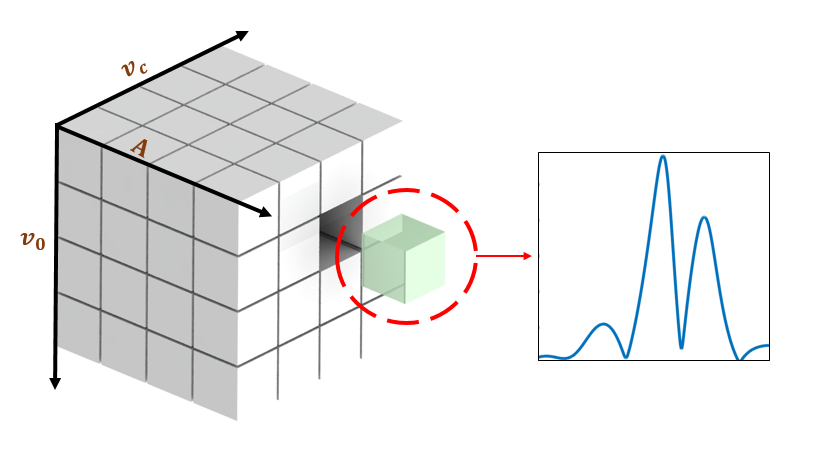
\includegraphics[width=0.7\textwidth]{fig/ch4_fig4.png}
        \caption{Concept schematic of look-up table used by accelerated scanned-WMS-$2f/1f$ spectral-fitting routine.}
    \label{fig:ch4_2}
\end{figure}


\section{Sensor Architecture}
\subsection{Experimental setup}

Fig. 4.3 illustrates a schematic of the experimental setup used to provide measurements of temperature and $H_2O$ concentration in a propane-air burner using the SE-LAS sensor. Two distributed-feedback (DFB) tunable diode lasers in a fiber pigtail configuration were multiplexed using a 2-by-2 fiber multiplexer. One arm of the fiber multiplexer was used to direct laser light to a conventional line-of-sight sensor (not shown here, see Fig. 4.7) and the other arm was connected to the fiber bundle utilized by the SE-LAS sensor. The fiber bundle was connected to the SE-LAS sensor housing (details provided in the following subsection) which was threaded directly into the wall of a stainless-steel propane-air burner. The burner has a 3" inner diameter and the inner surface of the burner has a matte finished (i.e., it is not polished). For the line-of-sight sensor, two NPT pipe plugs containing 0.5" diameter, sapphire windows were threaded into the burner wall. A type-$K$ thermocouple was used to monitor the burner’s exterior wall temperature adjacent to the SE-LAS sensor. The fiber bundle (Neptec OS) contains a single SMF-28 fiber (for transmitting laser light) which is surrounded by 6 multimode fibers (105 $\mu m$ core diameter, $NA=0.22$) for collecting the backscattered laser light and directing it to a photodetector. A lens doublet containing two aspheric lenses (Thorlabs C330TMD-C, $f=3.10 \,mm$, $d=6.33 \,mm$, $NA=0.68$) mounted in a cage system was used to collimate the light exiting the fiber bundle and focus it onto the detector (Thorlabs PDA10CS). The detector was operated with a gain of 30 $dB$, yielding a bandwidth of 775 $kHz$. The detector signal was recorded at 10 $MS/s$ on a 12 bit data acquisition card (GaGe CSE123G2).

 \begin{figure}[ht]
    \centering
        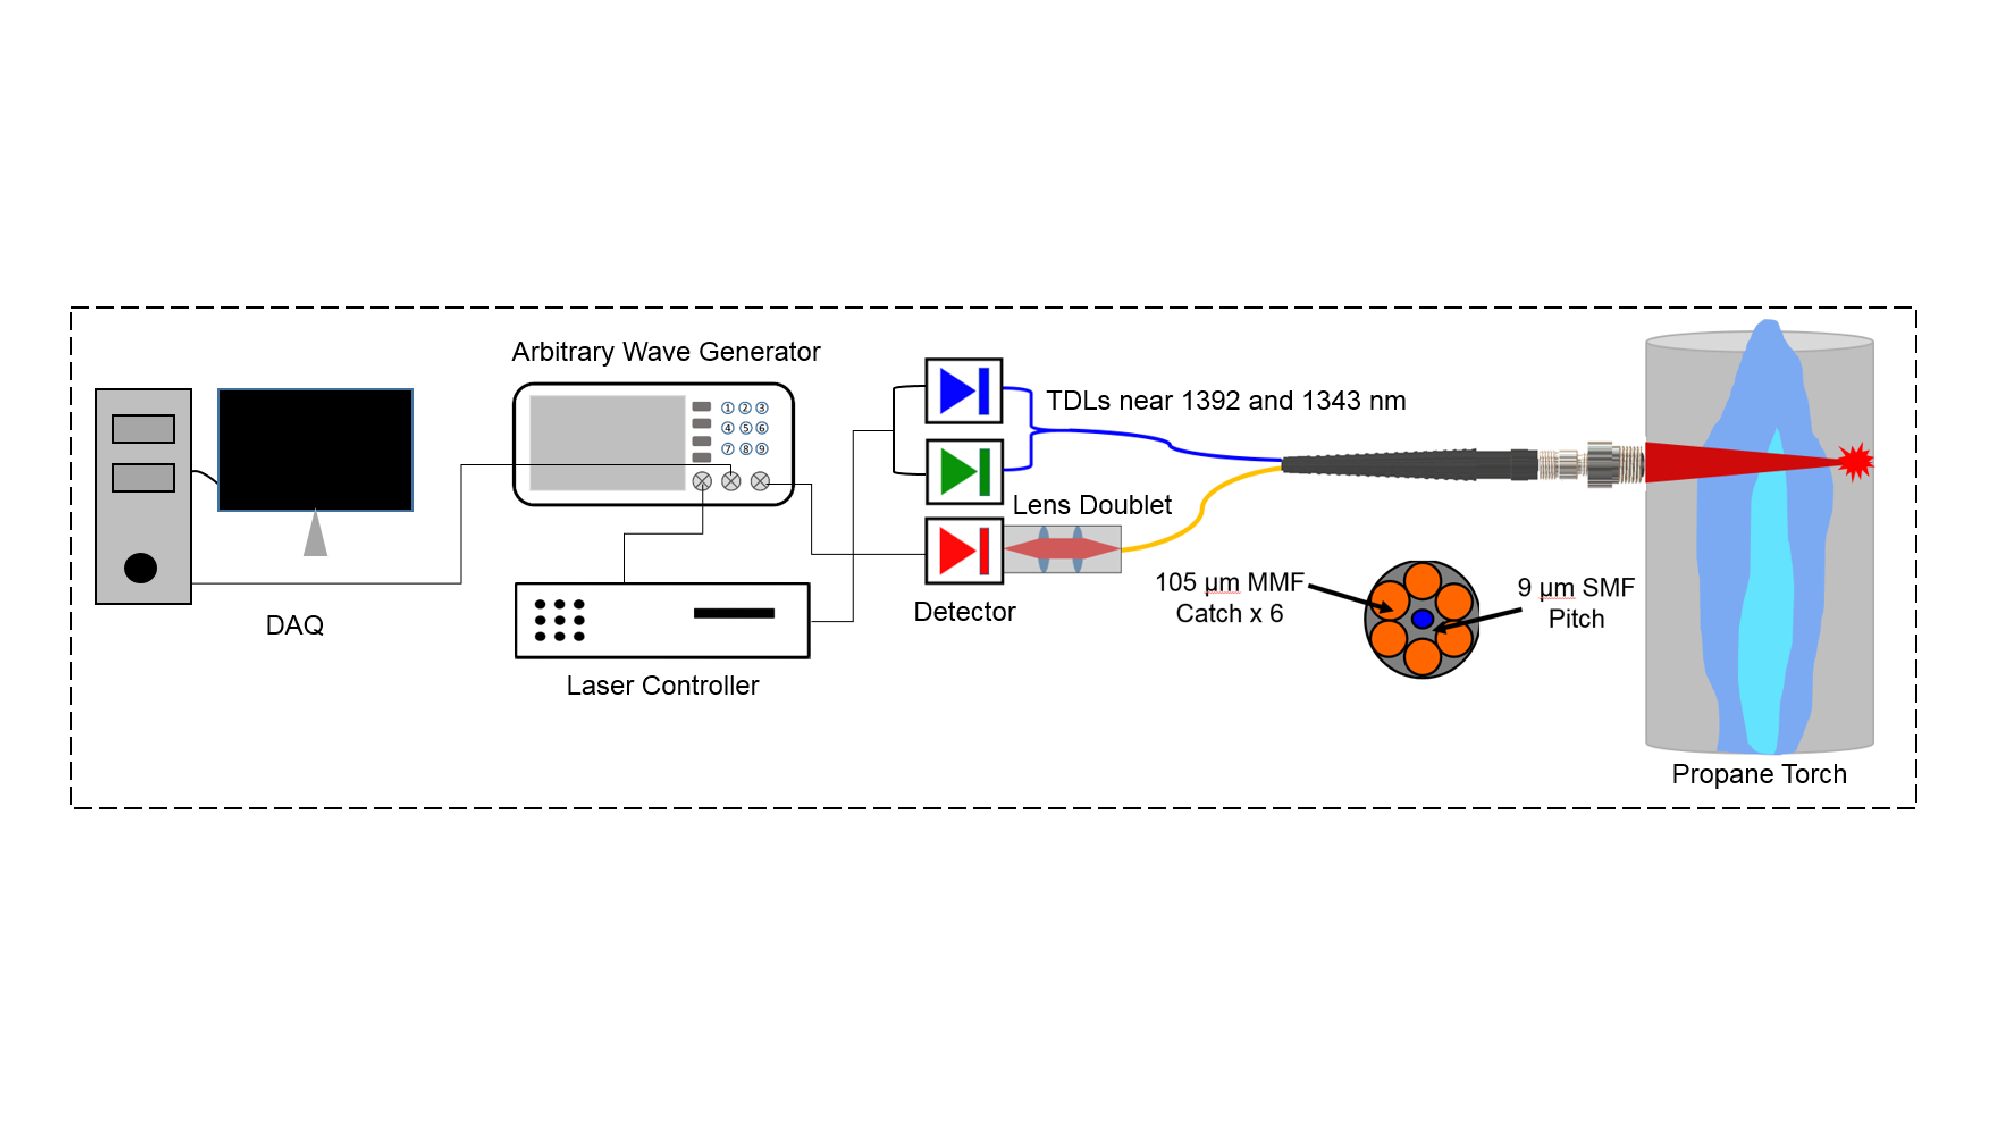
\includegraphics[trim = 0mm 52mm 0mm 20mm, clip=true, width=1\textwidth]{fig/ch4_fig1.pdf}
        \caption{Schematic of experimental setup used to measure temperature and $H_2O$ with the single-ended laser-absorption sensor.}
    \label{fig:ch4_3}
\end{figure}

The nominal temperature and current of the lasers were controlled by a commercially available laser controller (ILX Lightwave LDC3916372) and current modulation was achieved by applying a voltage modulation (generated by a 14-bit arbitrary waveform generator, Tektronix AFG 3252) to the modulation port on each laser’s controller card. During scanned-WMS experiments, the current of both lasers was scanned using a 1 $kHz$ sinewave while the laser near 1392 nm was modulated at 160 $kHz$ and the laser near 1343 nm was modulated at 200 $kHz$. The scan amplitude ($\sim 0.2 cm^{-1}$) was chosen to enable each laser to be scanned across their respective absorption transitions, and the modulation amplitudes (0.09 $cm^{-1}$ for 1392 $nm$ laser and 0.08 $cm^{-1}$ for 1343 $nm$ laser) were chosen to maximize the WMS-$2f$ signal of each laser at the nominal test conditions. The same modulation parameters were used in fixed-WMS experiments.


\subsection{Design of SE-LAS sensor housing}

 \begin{figure}[h]
    \centering
        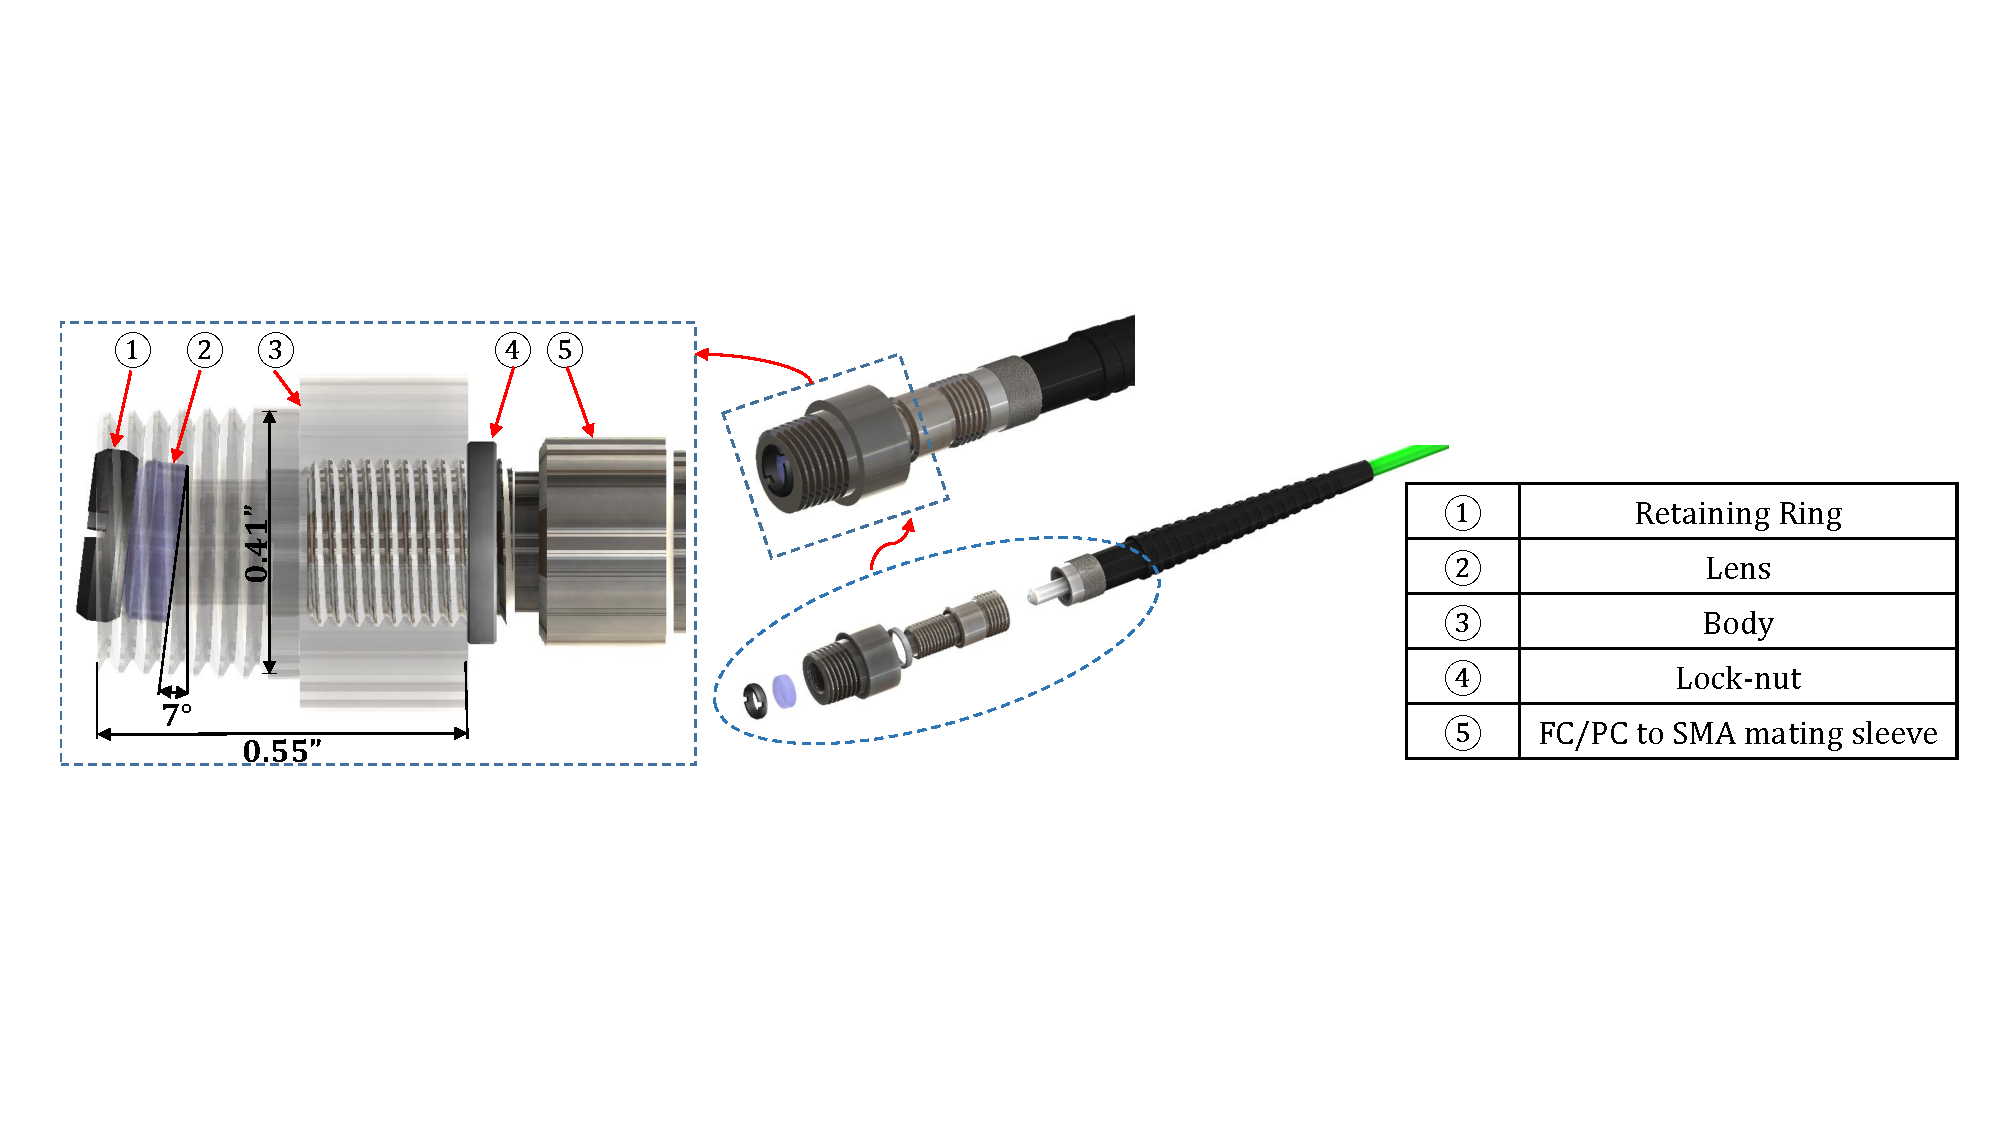
\includegraphics[trim = 0mm 52mm 0mm 20mm, clip=true, width=1\textwidth]{fig/ch4_fig2.pdf}
        \caption{CAD rendering of SE-LAS sensor housing and exploded view illustrating key components.}
    \label{fig:ch4_4}
\end{figure}


A CAD rendering illustrating the SE-LAS sensor housing is shown in Fig. 4.4. The sensor housing consists of: 1) a retaining ring with $M6.5\times 0.5$ threads (Thorlabs SM6RR), 2) an anti-reflection (AR) coated, BK7, plano-convex lens with a diameter of 6 mm and focal length of 15 $mm$ (Thorlabs: LA1222-C), 3) a custom stainless-steel body, 4) a lock-nut, and 5) a standard FC/PC to SMA mating sleeve (Thorlabs ADAFCSMA1). All parts, excluding the sensor body, are commercially available. The sensor body was custom made from a 316 stainless-steel rod and is 0.55" long with an outer diameter of 0.45". This sensor housing provides a 9$x$ smaller sensor footprint compared to that used in \cite{Goldenstein:16}. The sensor body has $1/8$" NPT external threads to enable convenient and sealed installation into the burner. The retaining ring ($M6.5 \times 0.5$ threads) was used to secure the lens to a shoulder tilted at $7^{\circ}$ relative to the optical axis in order to prevent collection of light reflected off the lens surface. The position of the fiber tip was adjusted to focus the laser light onto the target (i.e., the burner wall) which leads to maximum light collection efficiency \cite{Goldenstein:16}. Once the optimum location of the fiber tip was determined, the fiber position was locked in place using the lock-nut fastened to the FC/PC to SMA mating sleeve. Once locked in place, the SE-LAS sensor housing could be repeatedly removed and installed in the burner without compromising the light collection efficiency.


\subsection{SE-LAS Sensor design challenges}
Several design challenges were overcome to achieve a compact SE-LAS sensor that is suitable for direct exposure to high-temperature gases.

1. Miniaturize sensor housing: Reducing the size of the SE-LAS sensor housing introduced several design challenges which were addressed by careful selection of the lens parameters and housing dimensions. First, the distance between the fiber tip and lens was chosen such that the beam exiting the fiber does not diverge beyond the clear aperture of the system. This is required to ensure maximum optical throughput and prevent reflections within the sensor housing which could be collected by the fiber bundle and lead to unwanted background signals. This matter is further complicated by the fact that the distance between the lens and fiber tip must be chosen such that the lens focuses the transmitted light onto the scattering target to ensure maximum collection efficiency. As such, the focal length, clear aperture, and distance between fiber and lens must all be chosen together.
Second, miniaturizing the sensor housing corresponds to reducing the distance between the fiber tip and lens. This increases the amount of reflected light (off the lens surface) that is collected by the fiber bundle leading to unwanted background signals. This challenge was avoided here by mounting the lens on a shoulder that is tilted at $7^{\circ}$ relative to the optical axis, thereby directing the reflected beam outside the fiber bundle’s collection angle. It should be noted that this design element is necessary despite using an AR-coated lens with $\approx 0.3\%$ reflectance at the laser operating wavelengths. Using this arrangement, the amount of light that was reflected off the lens and collected by the fiber bundle was less than $0.5\%$ of that which was backscattered off the burner surface and collected.
Last, miniaturizing the sensor housing requires using a smaller lens which could reduce the amount of backscattered light that is collected by fiber bundle. However, despite using an 18$x$ smaller lens, our design provided a collection efficiency equal to 0.5 times that reported in \cite{Goldenstein:16} for a 15 $cm$ standoff distance. Given the similar optical design between these two SE-LAS sensors, this small difference in collection efficiency can be explained by recognizing that the fiber bundle accepts only a relatively small “cone” of backscattered light. As a result, using a larger lens does not provide much added benefit at the standoff distances studied here.

2. Extend sensor housing to high-temperature combustion environments: Several factors were considered to ensure that the SE-LAS could withstand direct exposure to high-temperature combustion gases for long durations. First, the lens must be able to withstand its peak operating temperature without melting or eroding in the presence of hot water vapor. This prohibits use of $CaF_2$ and other fluoride crystals which are hygroscopic and, thus, cannot withstand exposure to high-temperature water vapor as encountered here. Here, AR-coated BK7 was used due to its low cost ($\approx \$$30 USD), sufficiently high melting temperature ($\approx 830 \,K$), and ability to withstand exposure to hot water vapor. For higher-temperature and -pressure environments and/or mid-infrared applications, AR-coated sapphire lenses offer a better alternative due to its extremely high melting temperature ($\approx 2300\, K$), larger strength, resistance to thermal shock, and ability to tolerate hot combustion gases. However AR-coated sapphire lenses suitable for this SE-LAS sensor are not commercially available. Last, the body of the sensor housing should be constructed from a machinable material that has a relatively low thermal conductivity. This is required to insulate the fiber bundle from high temperatures since it is constructed using epoxy and plastics which cannot withstand temperatures greater than 150 C. Here, 316 stainless steel was used for the sensor body instead of aluminum due to its $\approx 15x$ smaller thermal conductivity. This was sufficient to prevent the FC/PC to SMA mating sleeve (i.e., the fiber bundle’s mating surface) from exceeding a temperature of 80 C. For higher-temperature environments, machinable ceramics may be a more suitable material.

3. Mitigate Cavity Noise: The SE-LAS sensor generates optical cavity noise since the incident and backscattered laser light overlap on each other and the optical coherence is sufficiently preserved after the reflection. As a result, during scanned-wavelength experiments, interference fringes can appear in the collected laser light as shown in \cite{Goldenstein:16}. To mitigate this noise source, WMS-$2f/1f$ is performed using modulation frequencies above 100 $kHz$ as recommended in \cite{Goldenstein:16}. Despite this added noise source and $100x$ lower optical throughput, the use of WMS-$2f/1f$ enables the SE-LAS sensor to provide measurements of temperature and $H_2O$ concentration with a comparable or better precision compared to a traditional line-of-sight-based LAS sensor (see Section 4.4.2).



\section{Experimental Results}
\subsection{Collection efficiency}
The collection efficiency of the SE-LAS sensor was measured as a function of standoff distance (i.e., working distance) for different reflectors/scattering targets to evaluate its optical design and operating limits. The distance between the SE-LAS sensor and aluminum (unpolished/mill finish with and without soot) and paper targets was varied by placing the SE-LAS sensor housing on a translation stage. A fiber-coupled power meter was used to measure both the optical power exiting the fiber bundle and the amount of backscattered optical power that was collected by the 6 MMF within the fiber bundle. Fig. 4.5 shows the fraction of light collected as a function of standoff distance. For the experiment and modulation setpoints used here, the quality of WMS-$2f/1f$ spectra degraded significantly when the fraction of light collected fell below $10^{-3}$. This coupled with the results shown in Fig. 4.5 indicates that the SE-LAS sensor (as presented here) should be capable of successful operation at standoff distances up to 100 $cm$. The fraction of light collected follows a power law decay (exponent near -1.7) with increasing standoff distance. The addition of soot (deposited using a rich propane flame) to the aluminum target (Fig. 4.6) reduced the fraction collected by only a factor of 5. This indicates that the SE-LAS sensor presented here should be robust against some degree of soot decomposition on combustor walls. Interestingly, for the clean aluminum target, teh SE-LAS sensor presented here yields a collection that is 50$\%$ (at $L=15$ $cm$) and 30$\%$ (at $L=100$ $cm$) of that shown in \cite{Goldenstein:16} where a 18$x$ larger lens (1" diameter) was used. However, for the paper target, the larger lens used in \cite{Goldenstein:16} yields a collection efficiency that is typically 10 times larger than that presented here. These results suggest that using a larger lens becomes increasingly more important as the standoff distance is increased or for backscattering targets that yield more diffuse reflections.

\vspace{3mm}

 \begin{figure}[h]
    \centering
        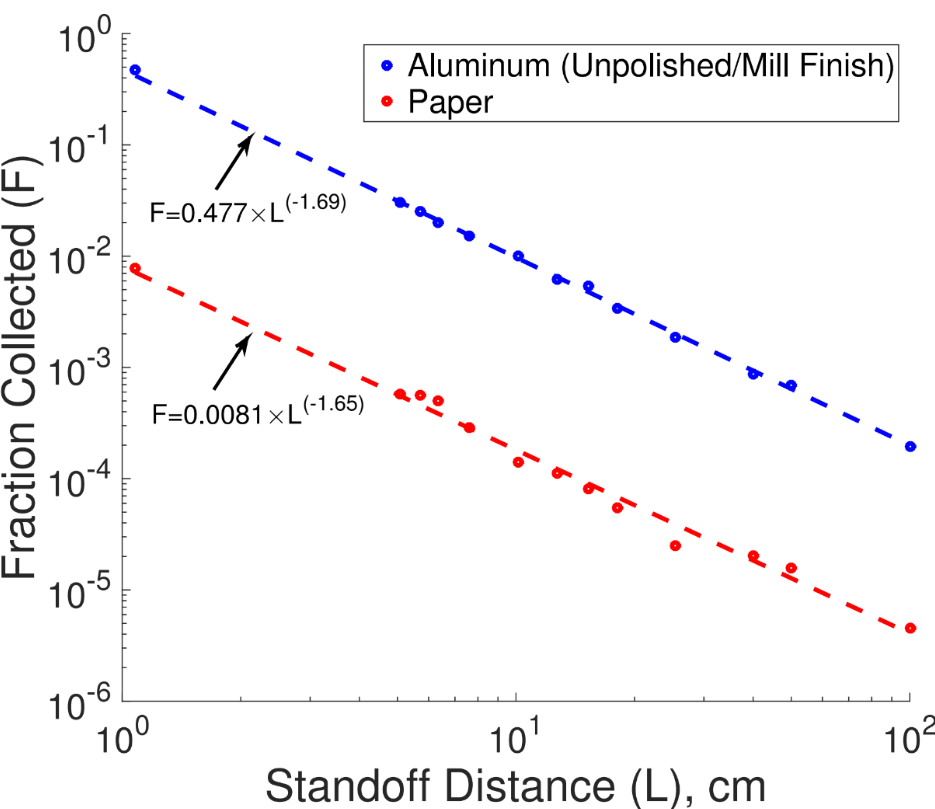
\includegraphics[width=0.5\textwidth]{fig/ch4_fig11_v2.png}
        \caption{Fraction of light collected by SE-LAS sensor as a function of standoff distance for aluminum and paper backscattering targets.}
    \label{fig:ch4_5}
\end{figure}

 \begin{figure}[h]
    \centering
        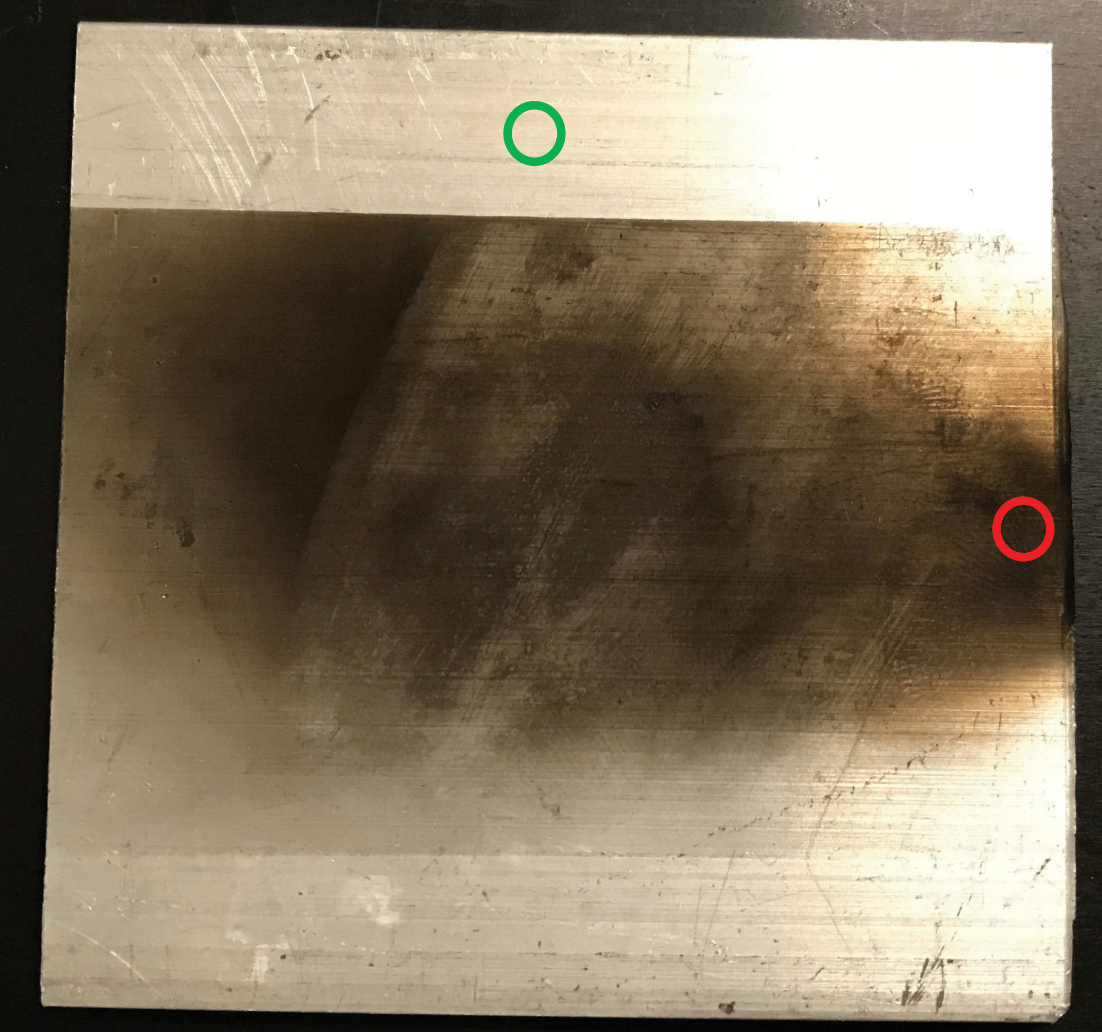
\includegraphics[width=0.4\textwidth]{fig/ch4_fig12.png}
        \caption{Photo of aluminum backscattering target. Green and red rings illustrate the laser beam location for comparing the fraction of light collected from backscattering off clean and soot-coated aluminum, respectively.}
    \label{fig:ch4_6}
\end{figure}


\subsection{Combustion experiments}
Experiments were conducted with the burner and LAS sensors operating in two modes: 1) Fixed-WMS experiments were conducted to resolve a transient ignition blast and 2) scanned-WMS experiments were conducted over a period of 30 minutes to monitor the quasi-steady behavior of the burner and proof-test the SE-LAS sensor in a high-temperature environment for a long duration. Fig. 4.7 illustrates the burner operating with both the line-of-sight LAS sensor and the single-ended LAS sensor installed on the burner body. Fig. 4.7(a) and Fig. 4.7(c) illustrate the burner during an ignition blast and the quasi-steady operation that follows, respectively.

 \begin{figure}[b]
    \centering
        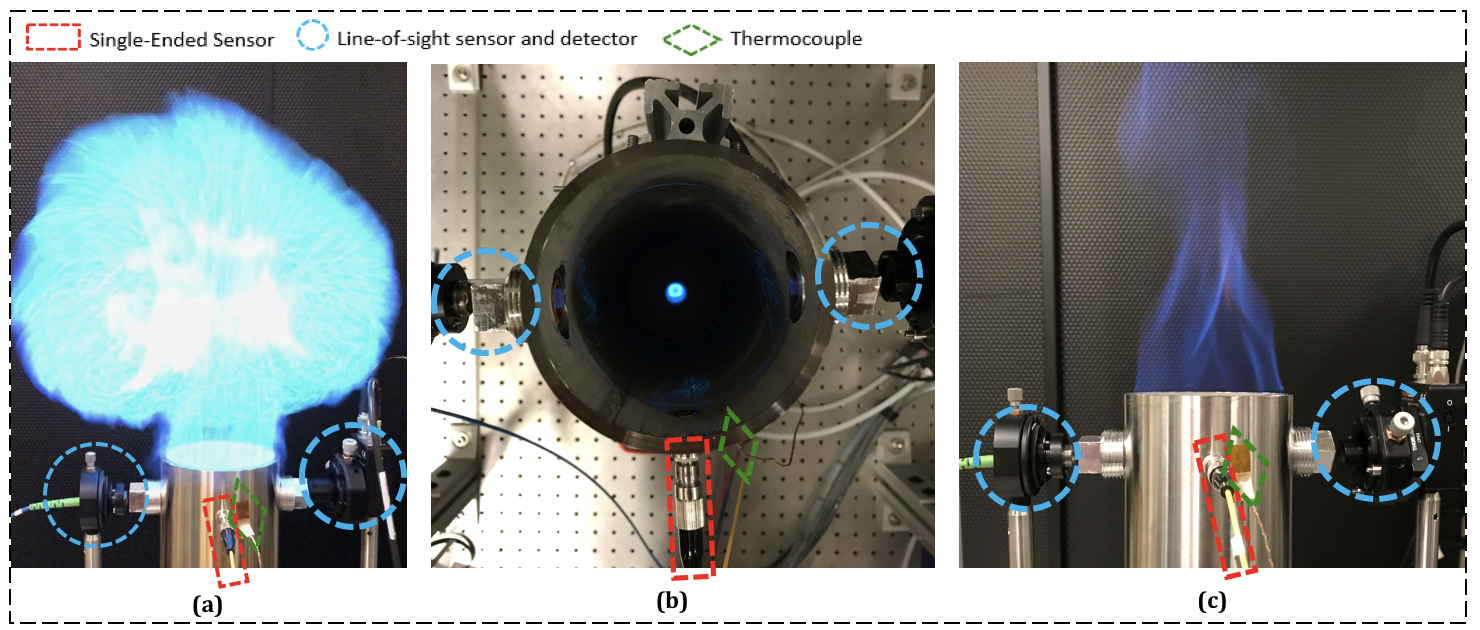
\includegraphics[width=1\textwidth]{fig/ch4_fig6_v3.png}
        \caption{Photos of propane-air burner during operation with LAS sensors and thermocouple installed. The photos illustrate the burner during an ignition blast (a), with a small throttled flame (b), and during quasi-steady state at full throttle (c).}
    \label{fig:ch4_7}
\end{figure}

Fig. 4.8 illustrates measured temperature time histories for both sensors during an ignition blast. The measurements were acquired using fixed-WMS-$2f/1f$ with 25 $kHz$ lock-in filters (applied during post-processing) to provide a measurement bandwidth of 25 $kHz$ (analogous to a 50 $kHz$ measurement rate). The results indicate excellent agreement between both sensors and suggest that the temperature field is axisymmetric during the test. The measured temperature time histories agree within 10 $K$ of each other and exhibit a $1\sigma$ precision of 22 $K$ (line-of-sight sensor) and 26 $K$ (single-ended sensor). These results suggest that our single-ended sensor offers comparable accuracy and precision to conventional line-of-sight sensors despite 100$x$ lower optical throughput (i.e., collection efficiency).

\begin{figure}[b]
    \centering
        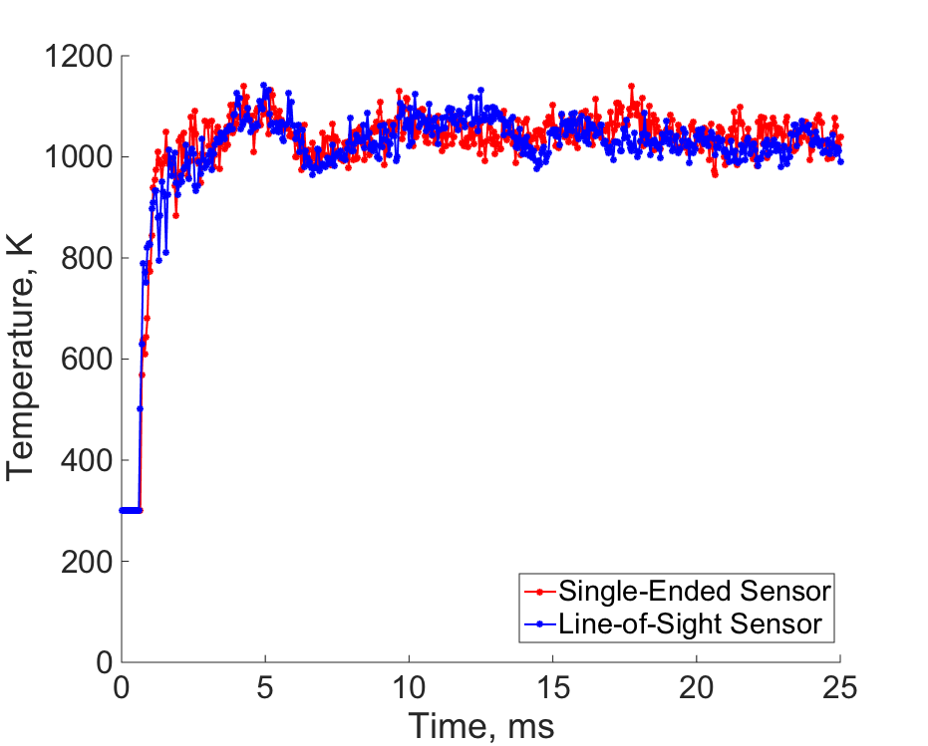
\includegraphics[width=0.6\textwidth]{fig/ch4_fig7.png}
        \caption{Temperature time histories measured during a burner ignition event using single-ended and line-of-sight LAS sensors and fixed-WMS-$2f/1f$ with a measurement bandwidth of 25 $kHz$.}
    \label{fig:ch4_8}
\end{figure}

\begin{figure} \centering 

\begin{subfigure}[b]{0.475\linewidth}  
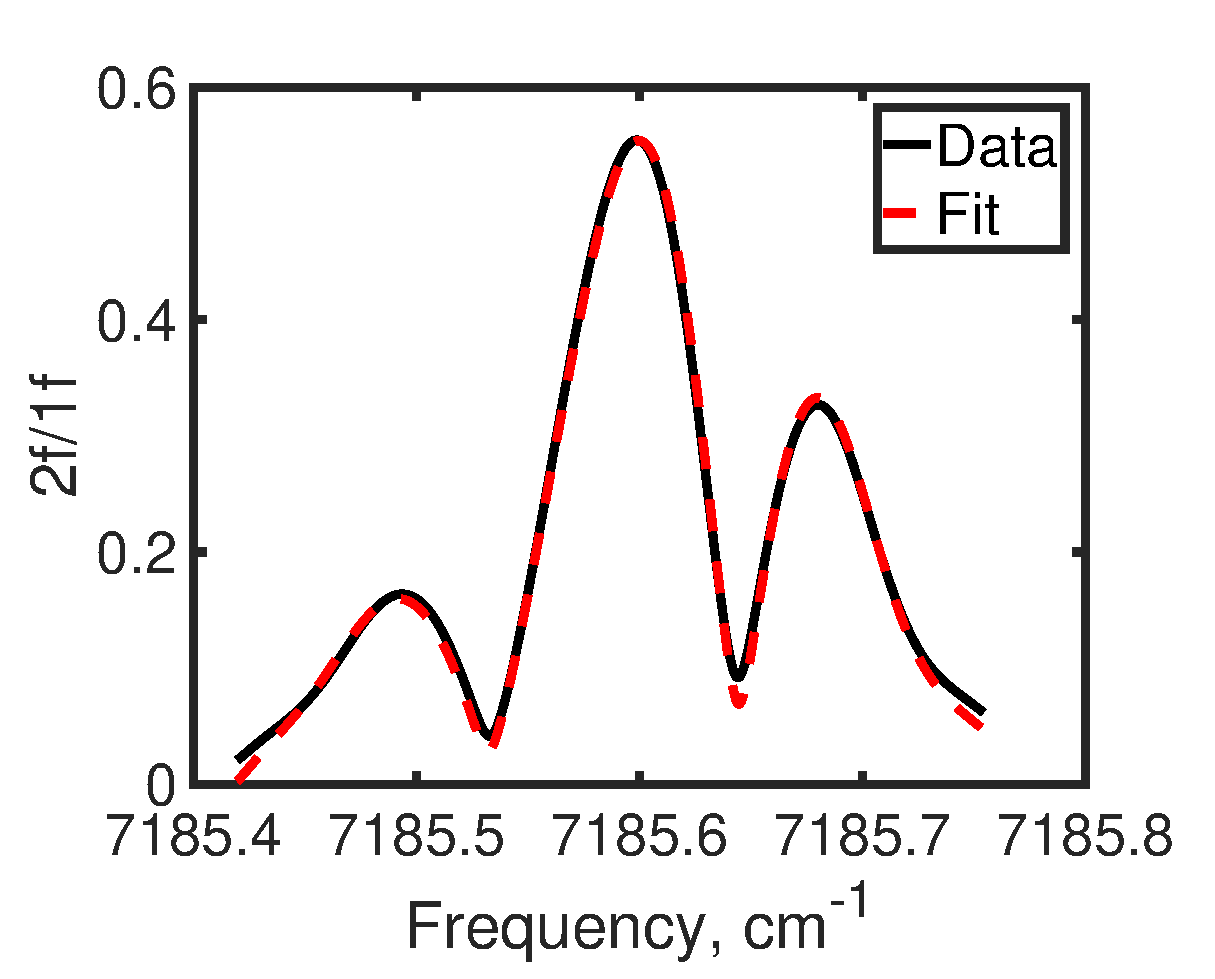
\includegraphics[width=\textwidth]{fig/LOS_1392_fit.eps}  
\end{subfigure}%  
\hfill
\begin{subfigure}[b]{0.475\linewidth}  
\centering  
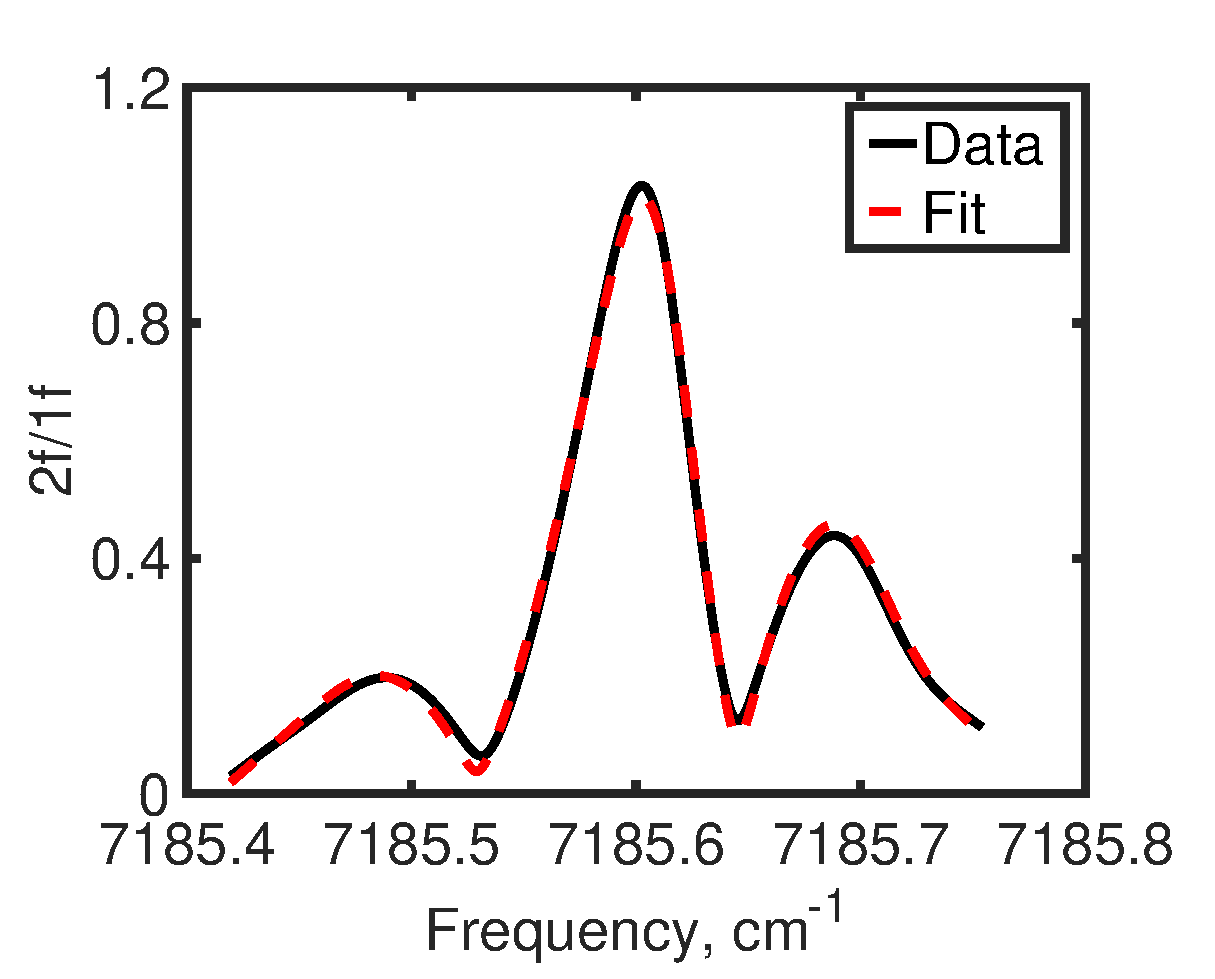
\includegraphics[width=\textwidth]{fig/SE_1392_fit.eps}  
\end{subfigure} 

\vskip\baselineskip
\begin{subfigure}[b]{0.475\linewidth}  
\centering  
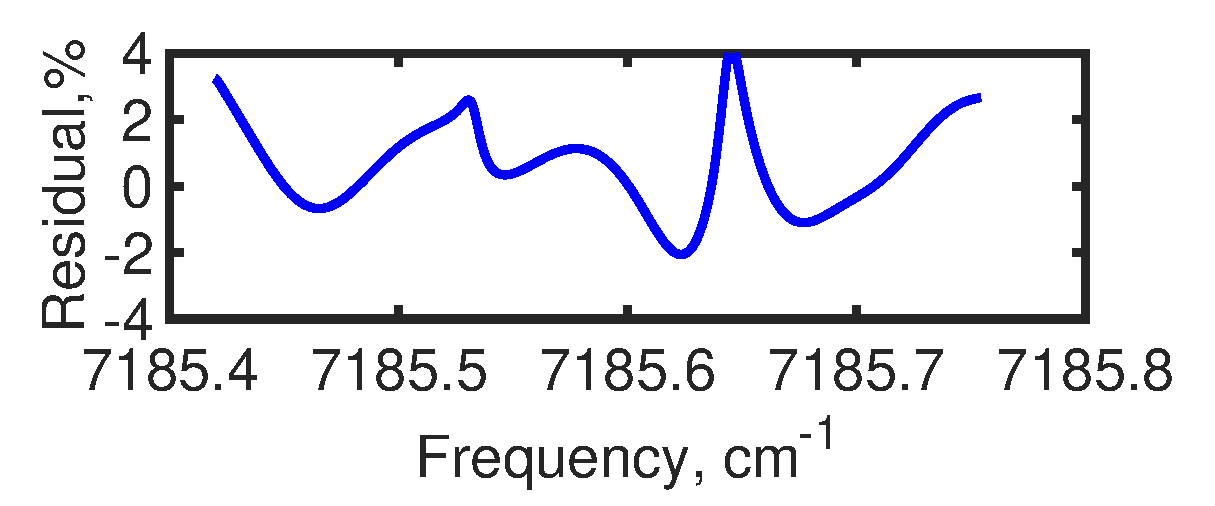
\includegraphics[width=\textwidth]{fig/LOS_1392_residual.eps}  
\caption{\underline{1392 nm: LOS}}
\end{subfigure} 
\quad
\begin{subfigure}[b]{0.475\linewidth}  
\centering  
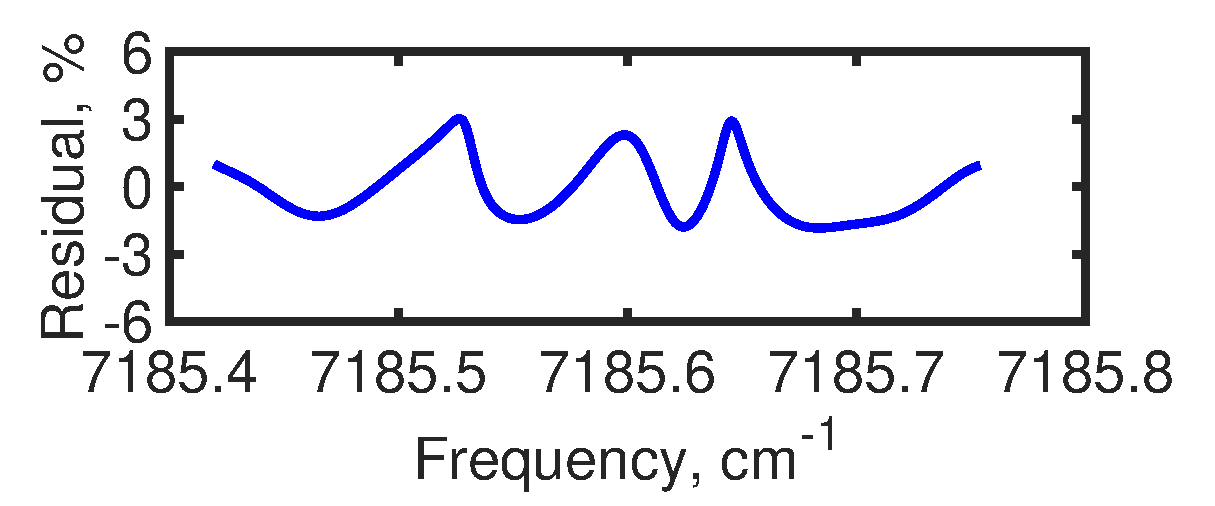
\includegraphics[width=\textwidth]{fig/SE_1392_residual.eps}  
\caption{\underline{1392 nm: SE}}
\end{subfigure} 

\begin{subfigure}[b]{0.475\linewidth}  
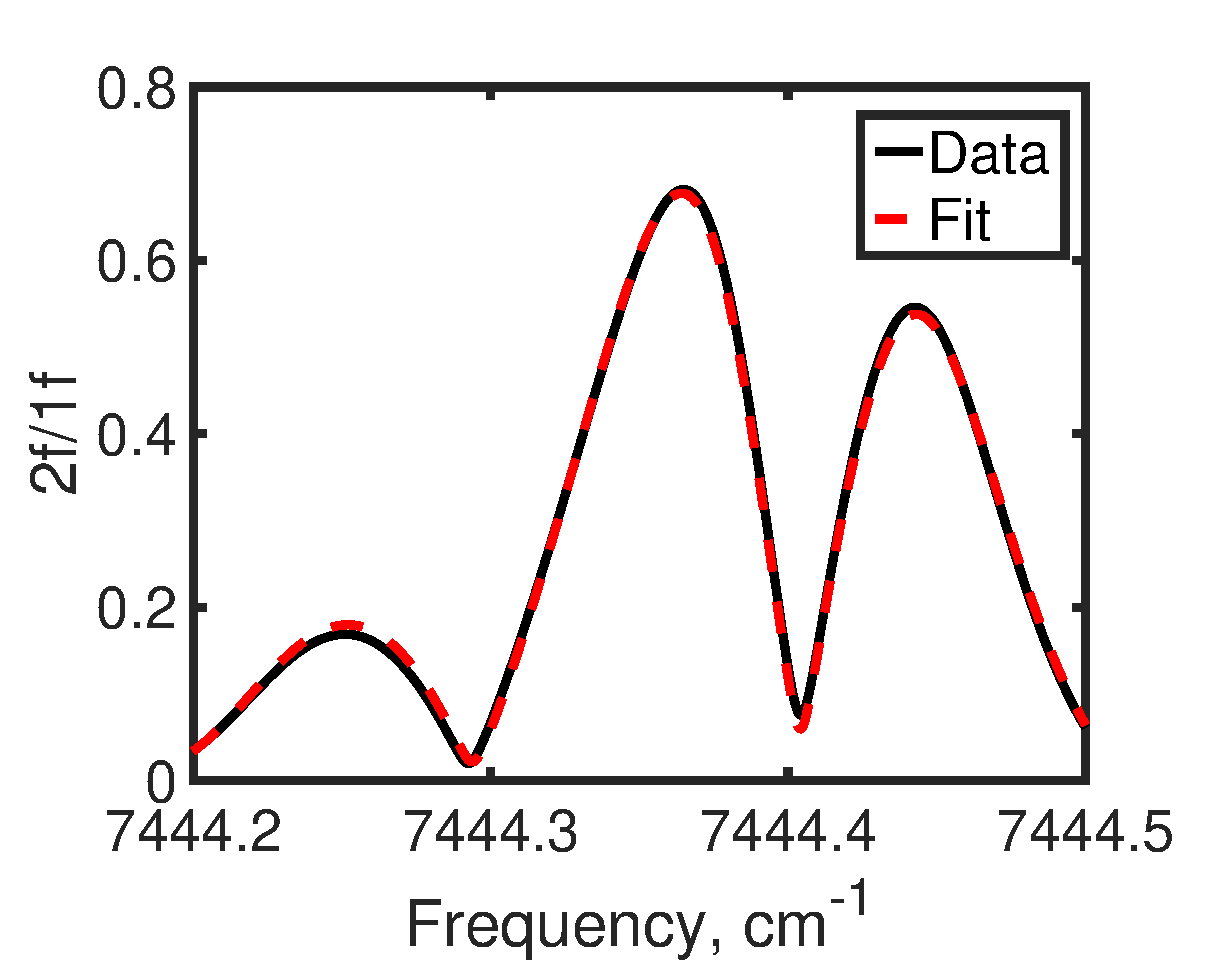
\includegraphics[width=\textwidth]{fig/LOS_1343_fit.eps}  
\end{subfigure}%  
\hfill
\begin{subfigure}[b]{0.475\linewidth}  
\centering  
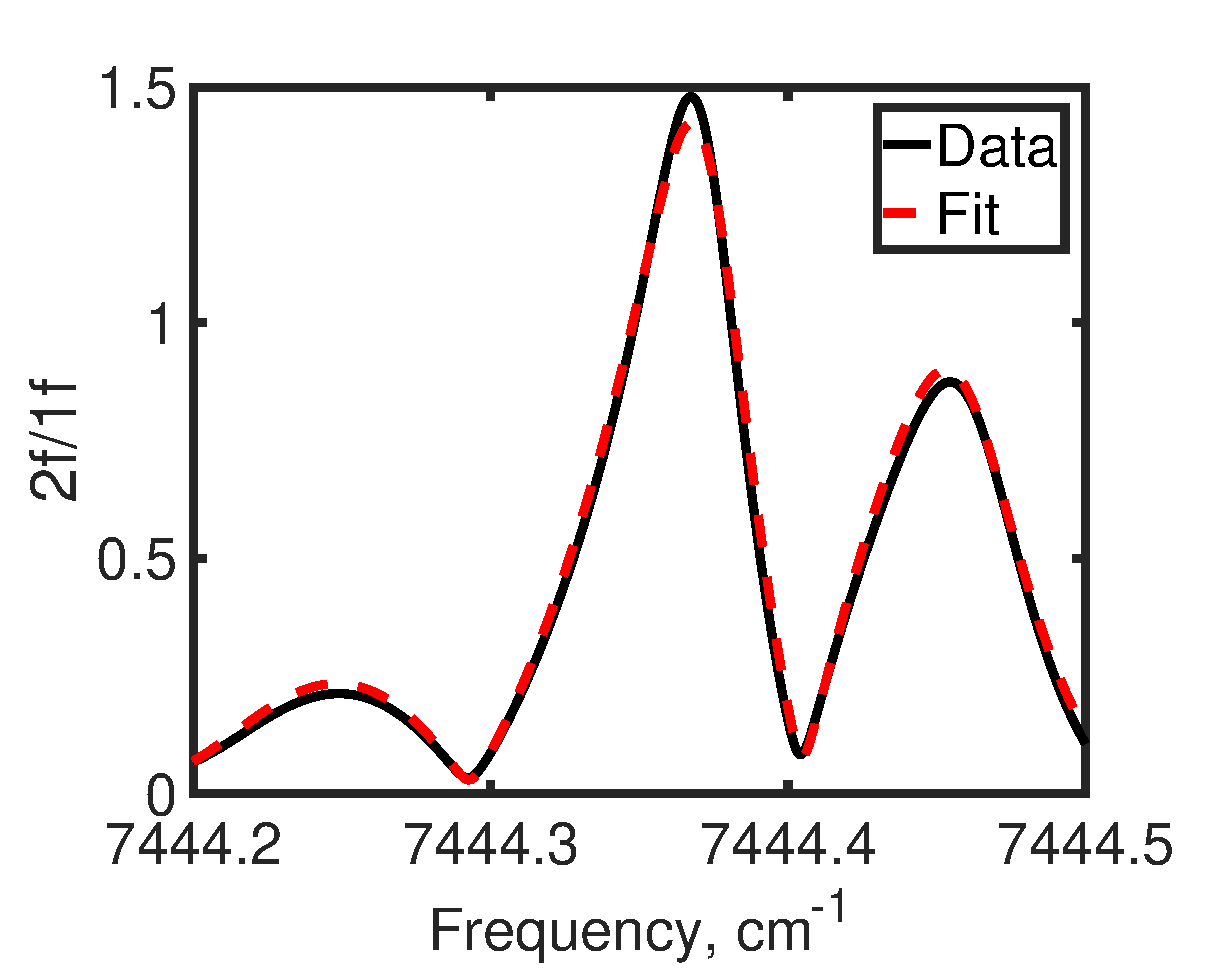
\includegraphics[width=\textwidth]{fig/SE_1343_fit.eps}  
\end{subfigure} 

\vskip\baselineskip
\begin{subfigure}[b]{0.475\linewidth}  
\centering  
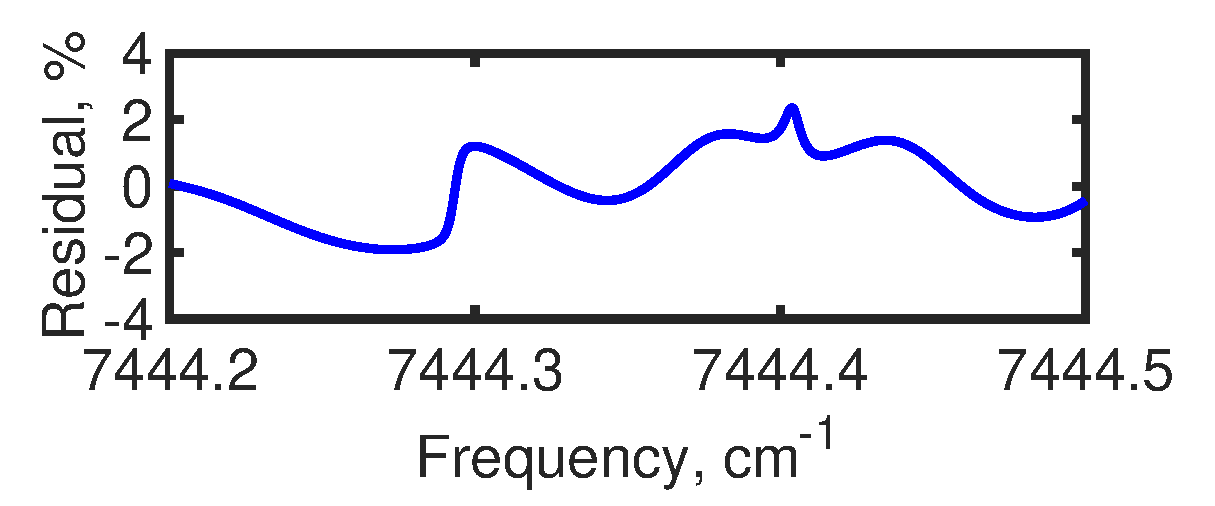
\includegraphics[width=\textwidth]{fig/LOS_1343_residual.eps}  
\caption{\underline{1343 nm: LOS}}
\end{subfigure} 
\quad
\begin{subfigure}[b]{0.475\linewidth}  
\centering  
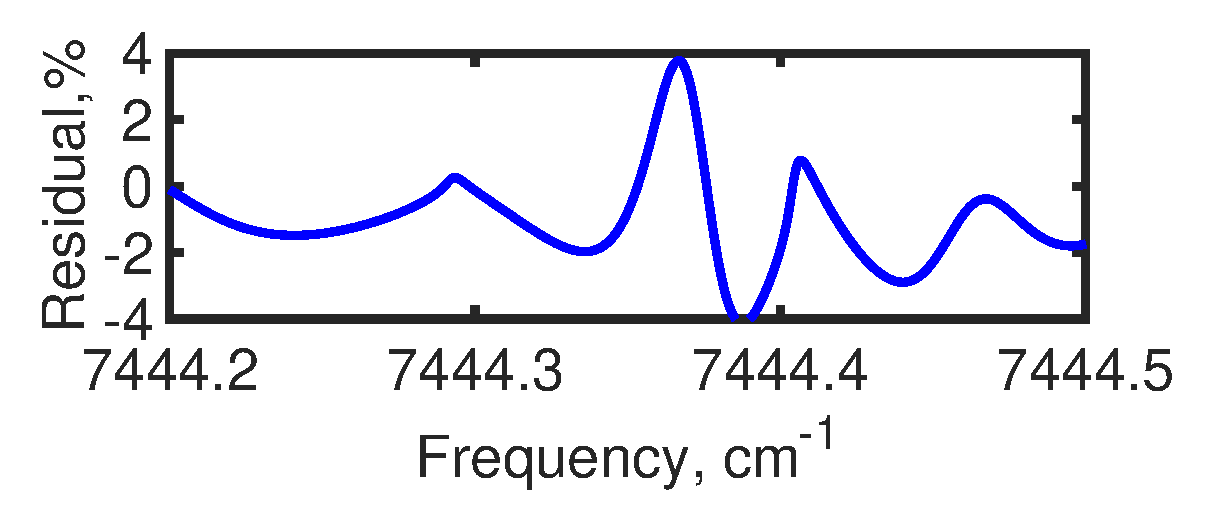
\includegraphics[width=\textwidth]{fig/SE_1343_residual.eps}  
\caption{\underline{1343 nm: SE}}
\end{subfigure} 

\caption{Example of measured and best-fit scanned-WMS-$2f/1f$ spectra for each laser and both LAS sensors (line-of-sight (LOS) and single-ended (SE)) with the burner operating at quasi-steady state.}
    \label{fig:ch4_8}
\end{figure}

Scanned-WMS-$2f/1f$ measurements of gas temperature and $H_2O$ mole fraction were acquired using the LOS- and SE-LAS sensors over a 30 minute period with the burner operating at quasi-steady state. This experiment was conducted to: 1) evaluate the performance of the SE-LAS sensor over an extended period of time in a high-temperature environment and 2) evaluate the accuracy and precision of the SE-LAS sensor while utilizing scanned-WMS-$2f/1f$ spectral fitting. To prevent excessive data collection, approximately 1 second of data was recorded once per minute for 30 minutes for each LAS sensor. The burner wall temperature was also recorded each minute to provide a conservative estimate for the temperature of the SE-LAS sensor’s lens and to establish when the burner walls reached a steady-state temperature. 

Fig. 4.9 illustrates a single scanned-WMS-$2f/1f$ spectrum and its best fit for each laser acquired using both the SE-LAS and LOS-LAS sensor with the burner operating at quasi-steady state (nominal gas conditions of approximately 1000 $K$ and 13$\%$ $H_2O$ by mole). The best-fit scanned-WMS-$2f/1f$ spectra were determined using the accelerated fitting routine described in Section 4.2.3. 


For both LAS sensors, the best-fit spectra provide peak-normalized residuals typically within $2\%$, although residuals as large as $4\%$ occur at isolated frequencies for the SE-LAS sensor. The performance of both sensors is consistent with that provided by previously developed line-of-sight-based sensors using scanned-WMS-2f/1f spectral fitting techniques \cite{Makowiecki2017,Goldenstein2014,goldenstein2014scanned,spearrin2014simultaneous}. These results indicate that our SE-LAS and accelerated scanned-WMS-$2f/1f$ spectral-fitting routine provide scanned-WMS-$2f/1f$ measurements of gas temperature and $H_2O$ mole fraction with an accuracy that is comparable to that of previously developed LAS sensors requiring optical access with an unobstructed line-of-sight.

For each one-second experiment, the accelerated scanned-WMS spectral-fitting routine was individually applied to all 2000 scanned-WMS-$2f/1f$ spectra (for each laser). The integrated absorbance corresponding to each best-fit spectrum was used to determine the gas temperature and $H_2O$ mole fraction at each moment in time as described in \cite{Goldenstein2014}. Fig. 4.10 shows a portion of a temperature and $H_2O$ mole fraction time history for both sensors.

\begin{figure} \centering 
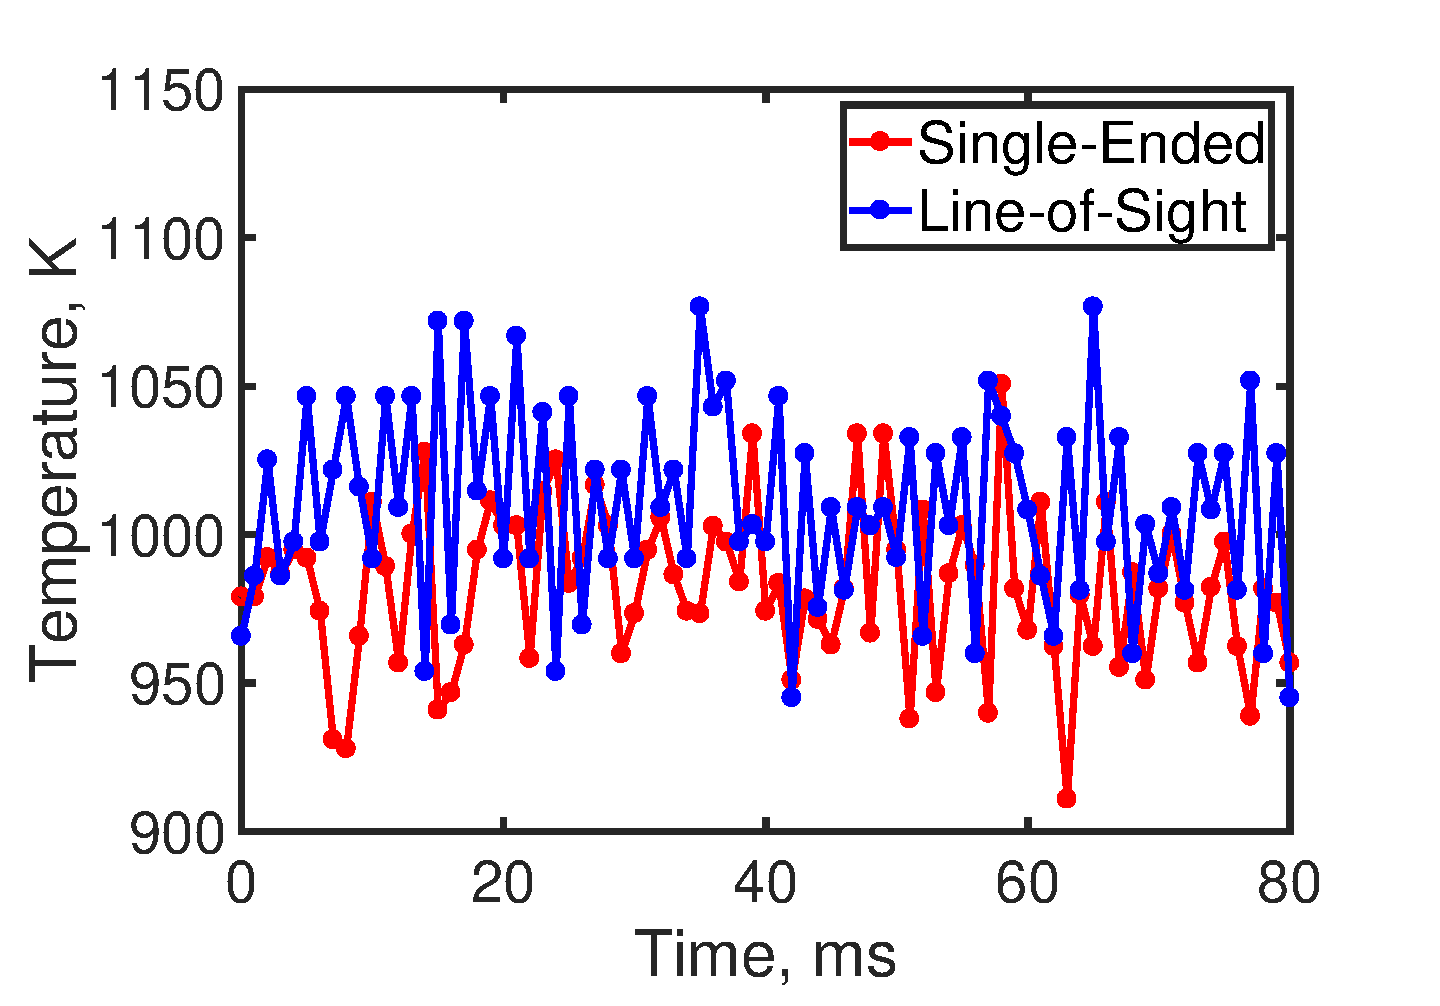
\includegraphics[width=0.7\textwidth]{fig/ch4_fig9_2.eps}  
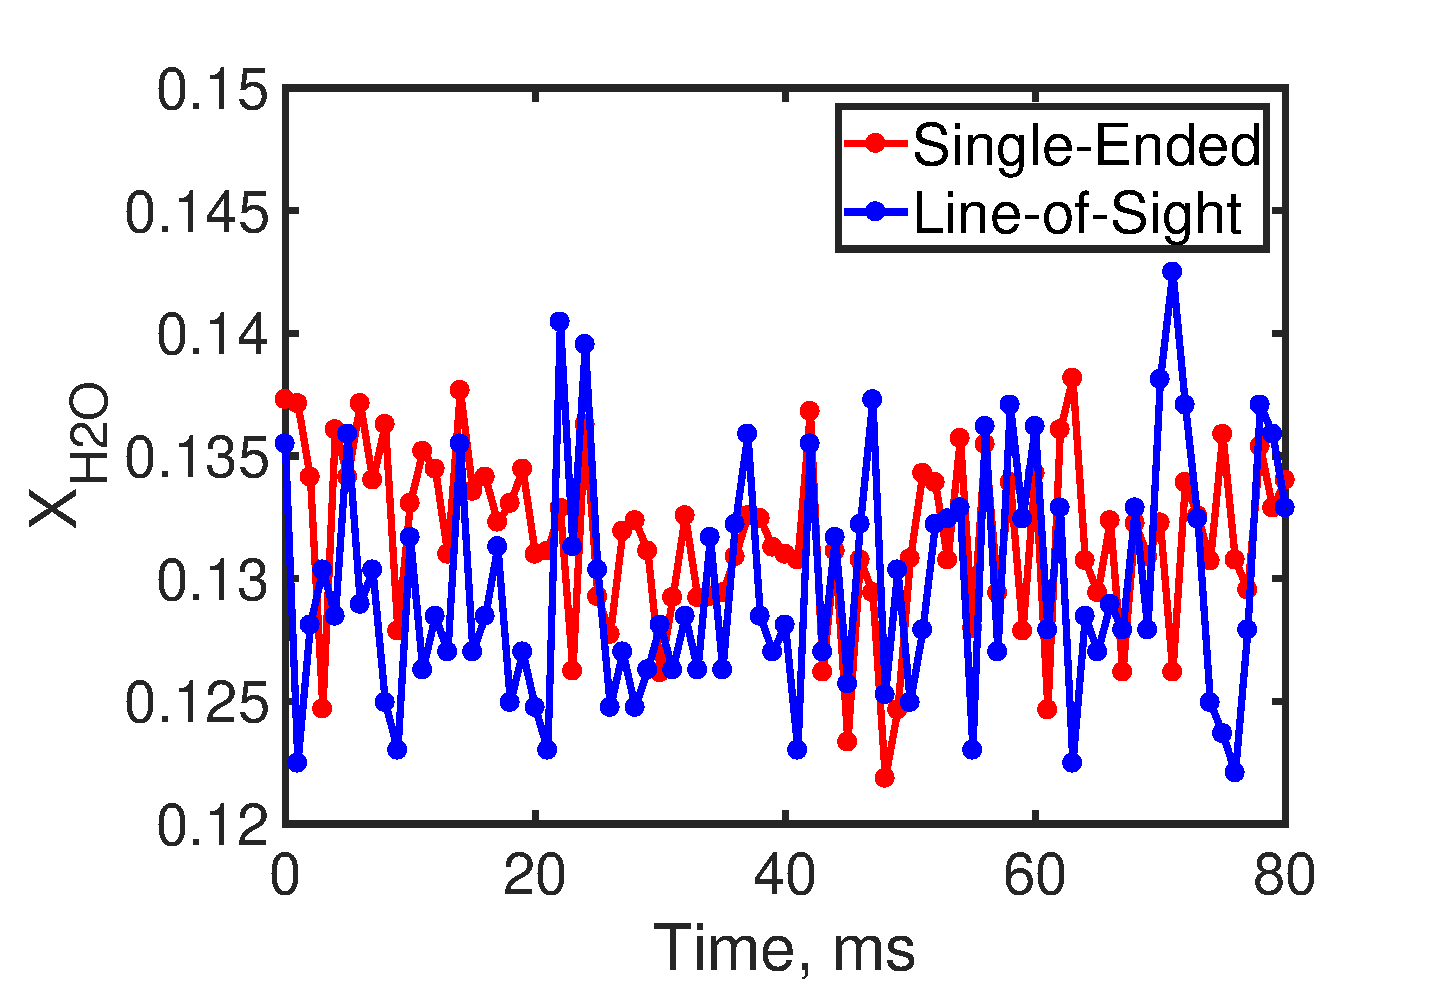
\includegraphics[width=0.7\textwidth]{fig/ch4_fig9_1.eps}  
\caption{Measurements of temperature and $H_2O$ mole fraction acquired at 2 kHz using both LAS sensors and the scanned-WMS-$2f/1f$ spectral fitting with the burner operating at quasi-steady state. Both sensors agree well and the SE-LAS sensor exhibits superior precision.}
    \label{fig:ch4_10}
\end{figure}



The temperature and $H_2O$ mole fraction time histories agree well between both sensors with a mean difference of 28.3 $K$ and 0.0005, respectively. Further, the SE-LAS sensor exhibited a superior $1\sigma$ measurement precision for temperature (26 $K$ compared to 32 $K$ for the LOS-LAS sensor) and $H_2O$ mole fraction (0.0037 compared to 0.0046 for LOS-LAS sensor). The improved precision of the SE-LAS sensor may result from its 2$x$ larger path length which leads to WMS-$2f/1f$ signals that are 2$x$ larger than those of the LOS-LAS sensor (see Fig. 4.9). 

\vspace{15mm}

\noindent The measured time histories illustrate that the gas temperature and $H_2O$ mole fraction are quasi-steady, however moderate fluctuations (compared to the precision observed during the ignition blast) between individual measurements exist. This likely results from swirl- and turbulence-induced fluctuations in combustion progress and heat transfer losses that have taken place leading up to the measurement plane. Visible imaging of the burner interior revealed pronounced swirling structures within the combustor which can also be observed by monitoring the flame at the burner exit plane (see Fig. 4.7(c)).

\begin{figure} \centering 
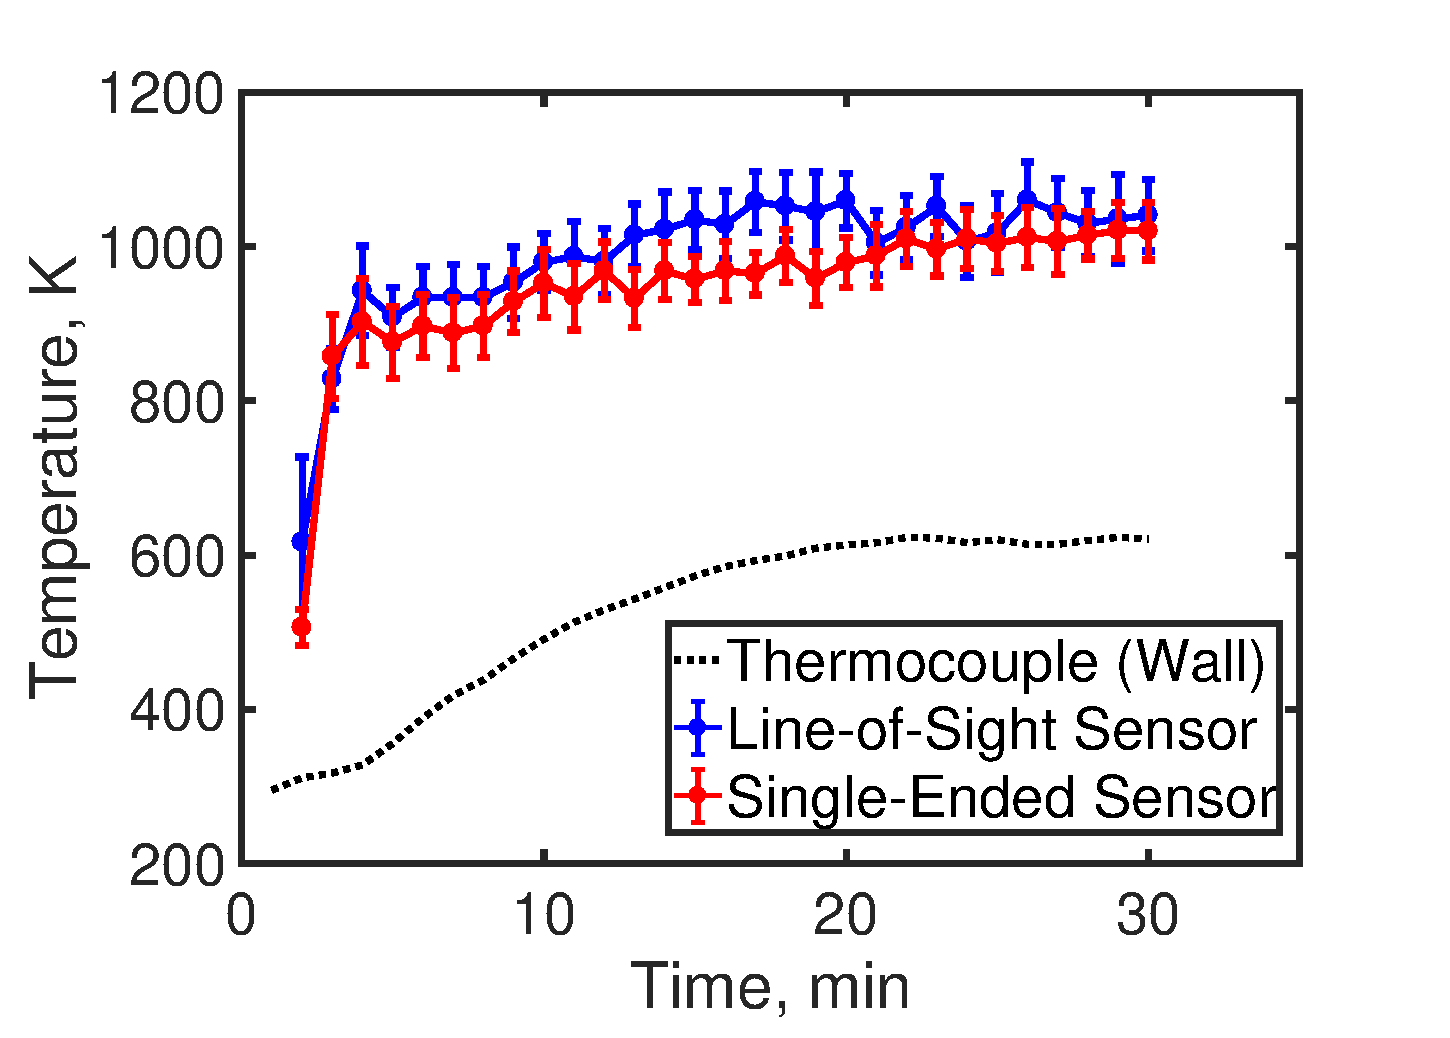
\includegraphics[width=0.7\textwidth]{fig/ch4_fig10_2.eps}  
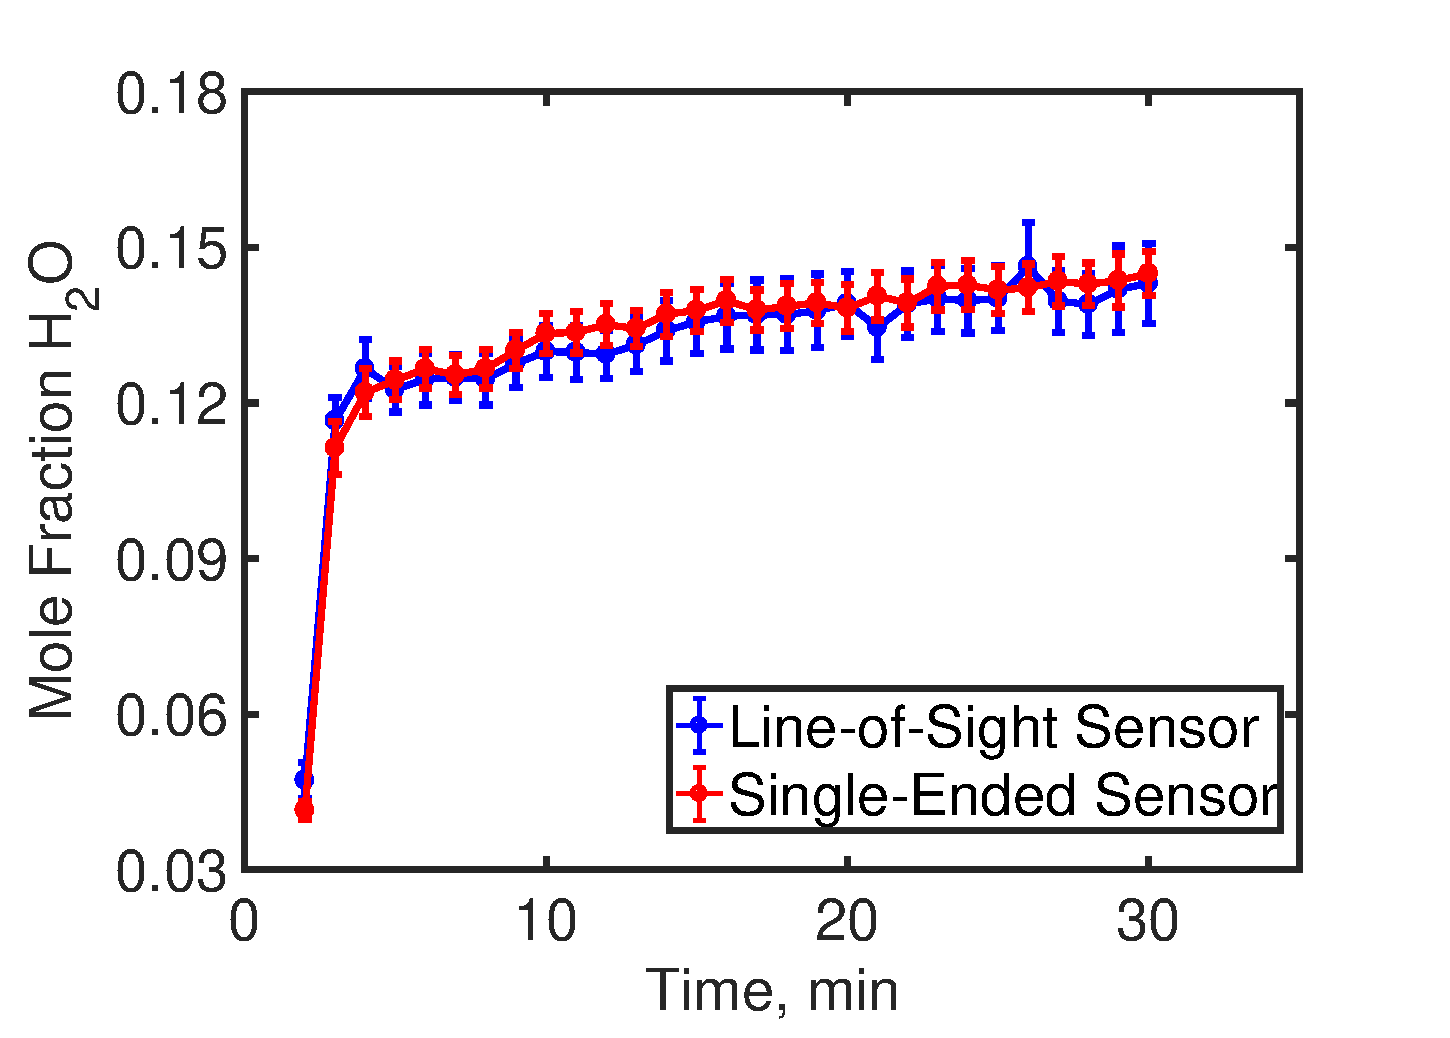
\includegraphics[width=0.7\textwidth]{fig/ch4_fig10_1.eps}  
\caption{Time-averaged (over 1 second) measurements of temperature (left) and $H_2O$ mole fraction (right) acquired using both LAS sensors over a 30 minute period with the burner operating at quasi-steady state. Error bars represent $1\sigma$ variation over each 1-second measurement period. The two LAS sensors agree well over the 30 minute test period and the SE-LAS sensor exhibits superior measurement precision.}
    \label{fig:ch4_10}
\end{figure}


Fig. 4.11 shows time-average (over one second) temperature and $H_2O$ mole fraction measurements acquired by both sensors over the complete 30-minute test period, as well as the burner wall temperature. The error bars represent the $1\sigma$ variation of each quantity within each one-second test. The first two experiments were conducted with the burner throttled to produce a small pilot flame (see Fig. 4.7(b)), and all of the following tests were conducted with the burner operating at full throttle to produce a large swirling flame that filled the burner and measurement path. The results indicate that the burner wall temperature reaches steady-state after 20 minutes and that the gas temperature and $H_2O$ mole fraction also increase slightly for the first 20 minutes of the test. These results can be explained by recognizing that heat transfer losses from the combustion gas will decrease as the burner wall temperature increases which will promote higher gas temperatures and reduce wall quenching. In general, the time-averaged gas temperature and $H_2O$ mole fraction measured by both LAS sensors agree within measurement precision, however the SE-LAS sensor typically recorded a slightly lower ($\approx \,10$-$20$ $K$) temperature. Given that the $H_2O$ mole fractions measured by both LAS sensors remained in agreement throughout the test, the difference in gas temperature is assumed to result from a non-axisymmetric temperature distribution across the measurement plane. This could result from non-axisymmetric heat transfer losses induced by the burner mounting hardware and windows employed by the LOS-LAS sensor.

Over the 30 minute test period the burner wall temperature rose to a temperature of 625 $K$, which provides a conservative estimate for the temperature reached by the SE-LAS sensor’s lens. In addition, the FC/PC to SMA mating sleeve reached a temperature of 80 $C$. The performance of the SE-LAS sensor did not degrade in any observable metric despite its components reaching such high temperatures and its lens being continually exposed to combustion gas at temperatures near 1000 $K$. Optical transmission did not degrade and nor did the signal-to-noise ratio of the WMS-$2f/1f$ signals. Since acquiring the experimental results presented here, similar long-duration experiments have been conducted repeatedly and the SE-LAS sensor has not shown any signs of degradation.
